%File: anonymous-submission-latex-2025.tex
\documentclass[letterpaper]{article} % DO NOT CHANGE THIS
\usepackage{aaai25}  % DO NOT CHANGE THIS
\usepackage{times}  % DO NOT CHANGE THIS
\usepackage{helvet}  % DO NOT CHANGE THIS
\usepackage{courier}  % DO NOT CHANGE THIS
\usepackage[hyphens]{url}  % DO NOT CHANGE THIS
\usepackage{graphicx} % DO NOT CHANGE THIS
\urlstyle{rm} % DO NOT CHANGE THIS
\def\UrlFont{\rm}  % DO NOT CHANGE THIS
\usepackage{natbib}  % DO NOT CHANGE THIS AND DO NOT ADD ANY OPTIONS TO IT
\usepackage{caption} % DO NOT CHANGE THIS AND DO NOT ADD ANY OPTIONS TO IT
\frenchspacing  % DO NOT CHANGE THIS
\setlength{\pdfpagewidth}{8.5in} % DO NOT CHANGE THIS
\setlength{\pdfpageheight}{11in} % DO NOT CHANGE THIS
%
% These are recommended to typeset algorithms but not required. See the subsubsection on algorithms. Remove them if you don't have algorithms in your paper.
\usepackage{algorithm}
\usepackage{algorithmic}
\usepackage{amsmath}
\usepackage{booktabs}
\usepackage{array}

%
% These are are recommended to typeset listings but not required. See the subsubsection on listing. Remove this block if you don't have listings in your paper.
\usepackage{newfloat}
\usepackage{listings}
\DeclareCaptionStyle{ruled}{labelfont=normalfont,labelsep=colon,strut=off} % DO NOT CHANGE THIS
\lstset{%
	basicstyle={\footnotesize\ttfamily},% footnotesize acceptable for monospace
	numbers=left,numberstyle=\footnotesize,xleftmargin=2em,% show line numbers, remove this entire line if you don't want the numbers.
	aboveskip=0pt,belowskip=0pt,%
	showstringspaces=false,tabsize=2,breaklines=true}
\floatstyle{ruled}
\newfloat{listing}{tb}{lst}{}
\floatname{listing}{Listing}
%
% Keep the \pdfinfo as shown here. There's no need
% for you to add the /Title and /Author tags.
\pdfinfo{
/TemplateVersion (2025.1)
}

% DISALLOWED PACKAGES
% \usepackage{authblk} -- This package is specifically forbidden
% \usepackage{balance} -- This package is specifically forbidden
% \usepackage{color (if used in text)
% \usepackage{CJK} -- This package is specifically forbidden
% \usepackage{float} -- This package is specifically forbidden
% \usepackage{flushend} -- This package is specifically forbidden
% \usepackage{fontenc} -- This package is specifically forbidden
% \usepackage{fullpage} -- This package is specifically forbidden
% \usepackage{geometry} -- This package is specifically forbidden
% \usepackage{grffile} -- This package is specifically forbidden
% \usepackage{hyperref} -- This package is specifically forbidden
% \usepackage{navigator} -- This package is specifically forbidden
% (or any other package that embeds links such as navigator or hyperref)
% \indentfirst} -- This package is specifically forbidden
% \layout} -- This package is specifically forbidden
% \multicol} -- This package is specifically forbidden
% \nameref} -- This package is specifically forbidden
% \usepackage{savetrees} -- This package is specifically forbidden
% \usepackage{setspace} -- This package is specifically forbidden
% \usepackage{stfloats} -- This package is specifically forbidden
% \usepackage{tabu} -- This package is specifically forbidden
% \usepackage{titlesec} -- This package is specifically forbidden
% \usepackage{tocbibind} -- This package is specifically forbidden
% \usepackage{ulem} -- This package is specifically forbidden
% \usepackage{wrapfig} -- This package is specifically forbidden
% DISALLOWED COMMANDS
% \nocopyright -- Your paper will not be published if you use this command
% \addtolength -- This command may not be used
% \balance -- This command may not be used
% \baselinestretch -- Your paper will not be published if you use this command
% \clearpage -- No page breaks of any kind may be used for the final version of your paper
% \columnsep -- This command may not be used
% \newpage -- No page breaks of any kind may be used for the final version of your paper
% \pagebreak -- No page breaks of any kind may be used for the final version of your paperr
% \pagestyle -- This command may not be used
% \tiny -- This is not an acceptable font size.
% \vspace{- -- No negative value may be used in proximity of a caption, figure, table, section, subsection, subsubsection, or reference
% \vskip{- -- No negative value may be used to alter spacing above or below a caption, figure, table, section, subsection, subsubsection, or reference

\setcounter{secnumdepth}{0} %May be changed to 1 or 2 if section numbers are desired.

% The file aaai25.sty is the style file for AAAI Press
% proceedings, working notes, and technical reports.
%

% Title

% Your title must be in mixed case, not sentence case.
% That means all verbs (including short verbs like be, is, using,and go),
% nouns, adverbs, adjectives should be capitalized, including both words in hyphenated terms, while
% articles, conjunctions, and prepositions are lower case unless they
% directly follow a colon or long dash




% REMOVE THIS: bibentry
% This is only needed to show inline citations in the guidelines document. You should not need it and can safely delete it.
%\usepackage{bibentry}
% END REMOVE bibentry

\begin{document}

\title{EasyInv: Toward Fast and Better DDIM Inversion}
\author {
    Ziyue Zhang\textsuperscript{\rm 1},
    Mingbao Lin\textsuperscript{\rm 2},
    Shuicheng Yan\textsuperscript{\rm 2},
    Rongrong Ji\textsuperscript{\rm 1}
}
\affiliations {
    \textsuperscript{\rm 1}Key Laboratory of Multimedia Trusted Perception and Efficient Computing, Ministry of Education of China, Xiamen University, China\\
    \textsuperscript{\rm 2}Skywork AI, Singapore\\
    zhang\_zi\_yue@foxmail.com, linmb001@outlook.com, shuicheng.yan@kunlun-inc.com, rrji@xmu.edu.cn
}

\maketitle

\begin{abstract}
This paper introduces EasyInv, an easy yet novel approach that significantly advances the field of DDIM Inversion by addressing the inherent inefficiencies and performance limitations of traditional iterative optimization methods.
%
At the core of our EasyInv is a refined strategy for approximating inversion noise, which is pivotal for enhancing the accuracy and reliability of the inversion process.
%
By prioritizing the initial latent state, which encapsulates rich information about the original images, EasyInv steers clear of the iterative refinement of noise items. 
%
Instead, we introduce a methodical aggregation of the latent state from the preceding time step with the current state, effectively increasing the influence of the initial latent state and mitigating the impact of noise.
%
We illustrate that EasyInv is capable of delivering results that are either on par with or exceed those of the conventional DDIM Inversion approach, especially under conditions where the model's precision is limited or computational resources are scarce. Concurrently, our EasyInv offers an approximate threefold enhancement regarding inference efficiency over off-the-shelf iterative optimization techniques.
\end{abstract}

% Uncomment the following to link to your code, datasets, an extended version or similar.
%
% \begin{links}
%     \link{Code}{https://aaai.org/example/code}
%     \link{Datasets}{https://aaai.org/example/datasets}
%     \link{Extended version}{https://aaai.org/example/extended-version}
% \end{links}

\section{Introduction}
\label{Intro}
%
%
Diffusion models have become a major focus of research in recent years, mostly renowned for their ability to generate high-quality images that closely match given prompts. Among the many diffusion models introduced in the community, Stable Diffusion (SD)~\cite{rombach2022high} stands out as one of the most widely utilized in scientific research, largely due to its open-source nature. Another contemporary diffusion model gaining popularity is DALL-E 3~\cite{betker2023improving}, which offers users access to its API and the ability to interact with it through platforms like ChatGPT~\cite{chatGPT}.
%
These models have significantly transformed the visual arts industry and have attracted substantial attention from the research community. 
%
%By providing tools for generating highly detailed and accurate images, they have opened new avenues for creative expression and technical innovation. 
%
%Nowadays, researchers and artists are leveraging these models to push the boundaries of what is possible in digital art and automated image synthesis. The integration of these models into various platforms underscores their versatility and growing importance in both academic and practical applications.



While renowned generative diffusion models have made significant strides, a prevalent limitation is their reliance on textual prompts for input.
%
This approach becomes restrictive when users seek to iteratively refine an image, as the sole reliance on prompts hinders flexibility.
%
Although solutions such as ObjectAdd~\cite{zhang2024objectadd} and P2P~\cite{hertz2022prompt} have been proposed to address image editing challenges, they are still confined to the realm of prompted image manipulation.
%
Given that diffusion models generate images from noise inputs, a potential breakthrough lies in identifying the corresponding noise for any given image.
%
This would enable the diffusion model to initiate the generation process from a known starting point, thereby allowing for precise control over the final output.
%
The recent innovation of DDIM Inversion~\cite{couairon2023diffedit} aims to overcome this challenge by reversing the denoising process to introduce noise.
%
This technique effectively retrieves the initial noise configuration after a series of reference steps, thereby preserving the integrity of the original image while affording the user the ability to manipulate the output by adjusting the denoising parameters.
%
With DDIM inversion, the generative process becomes more adaptable, facilitating the creation and subsequent editing of images with greater precision and control.
%
For example, the MasaCtrl method~\cite{cao_2023_masactrl} first transforms a real image into a noise representation and then identifies the arrangement of objects during the denoising phase.
%
Portrait Diffusion\cite{liu2023portrait} simultaneously inverts both the source and target images. Subsequently, it merges their respective $Q$, $K$ and $V$ values for mixups.


\begin{figure}
  \centering
  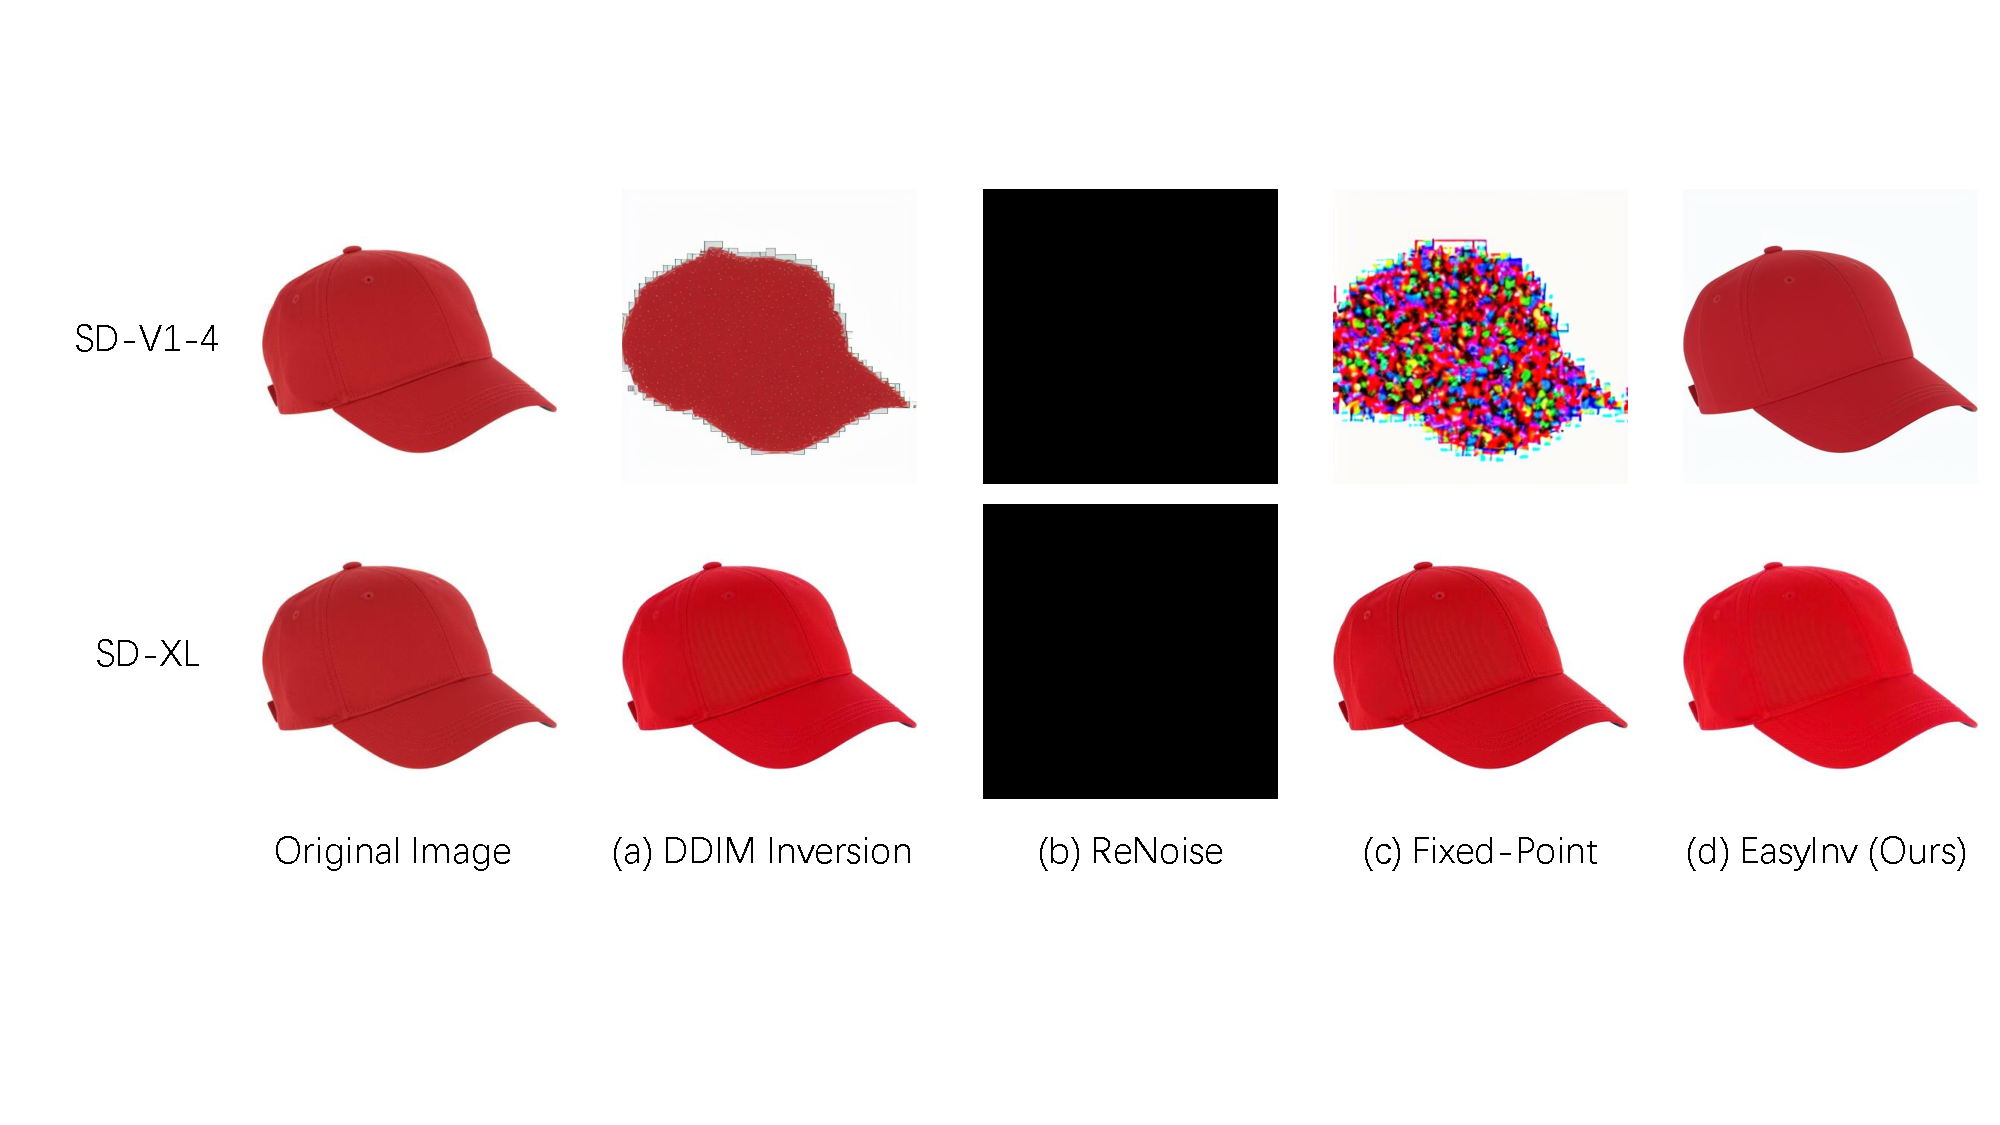
\includegraphics[width=0.98\linewidth]{visual_hat_result_together_cut.pdf}
  \caption{Performance comparison of inversion methods including vanilla DDIM Inversion~\cite{couairon2023diffedit}, Fixed-Point Iteration~\cite{pan2023effective}, ReNoise~\cite{garibi2024renoise} and our EasyInv. The proposed EasyInv performs well upon different diffusion models of SD-V1-4 and SD-XL.}
  \label{fig_inver}
\end{figure}



%
Considering the reliance on inversion techniques to preserve the integrity of the input image, the quality of the inversion process is paramount, as it profoundly influences subsequent tasks.
%
%
As depicted in Figure \ref{fig_inver}(a), the performance of DDIM Inversion has been found to be less than satisfactory due to the discrepancy between the noise estimated during the inversion process and the noise expected in the sampling process.
%
Consequently, numerous studies have been conducted to enhance its efficacy.
%
In Null-Text inversion~\cite{mokady2023null}, researchers observed that using a null prompt as input, the diffusion model could generate optimal results during inversion, suggesting that improvements to inversion might be better achieved in the reconstruction branch.
%
Ju \emph{et al}.'s work~\cite{ju2023direct} exemplifies this approach by calculating the distance between latents at the current step and the previous step.
%
PTI~\cite{dong2023prompt} opts to update the conditional vector in each step to guide the reconstruction branch for improving consistency.
%
ReNoise~\cite{garibi2024renoise} focuses on refining the inversion process itself. This method iteratively adds and then denoises noise at each time step, using the denoised noise as input for the subsequent iteration. However, as shown in Figure \ref{fig_inver}(b), it can result in a black image output when dealing with certain special inputs, which will be discussed in detail in Sec.\,\ref{exp}.
%
Pan \emph{et al.}~\cite{pan2023effective}, while maintaining the iterative updating process, also amalgamated noise from previous steps with the current step's noise. However, this method's performance is limited in less effective models as displayed in Figure\ref{fig_inver}(c). For instance, it performs well in SD-XL~\cite{podell2023sdxl} but fails to yield proper results in SD-V1-4~\cite{rombach2022high}. We attribute this to their method's sole focus on optimizing noise; when the noise is highly inaccurate, such simple optimization strategies encounter difficulties. Additionally, the iterative updating of noise is time-consuming, as Pan \emph{et al.}'s method requires multiple model inferences per time step.

In this paper, we conduct an in-depth analysis and recognize that the foundation of any inversion process is the initial latent state derived from a real image. Errors introduced at each step of the inversion process can accumulate, leading to a suboptimal reconstruction. Current methodologies, which focus on optimizing the transition between successive steps, may not be adequate to address this issue holistically. To tackle this, we propose a novel approach that considers the inversion process as a whole, underscoring the significance of the initial latent state throughout the process. Our approach, named EasyInv, incorporates a straightforward mechanism to periodically reinforce the influence of the initial latent state during the inversion. This is realized by blending the current latent state with the previous one at strategically selected intervals, thereby increasing the weight of the initial latent state and diminishing the noise's impact. As a result, EasyInv ensures a reconstructed version that remains closer to the original image, as illustrated in Figure\,\ref{fig_inver}(d). Furthermore, by building upon the traditional DDIM Inversion framework~\cite{couairon2023diffedit}, EasyInv does not depend on iterative optimization between adjacent steps, thus enhancing computational efficiency. In Figure\,\ref{fig_mid_step}, we present a visualization of the latent states at the midpoint of the total denoising steps for various inversion methods. It is evident that the outcomes of our EasyInv are more closely aligned with the original image compared to all other methods, demonstrating that EasyInv achieves faster convergence.




\begin{figure}[!t]
  \centering
  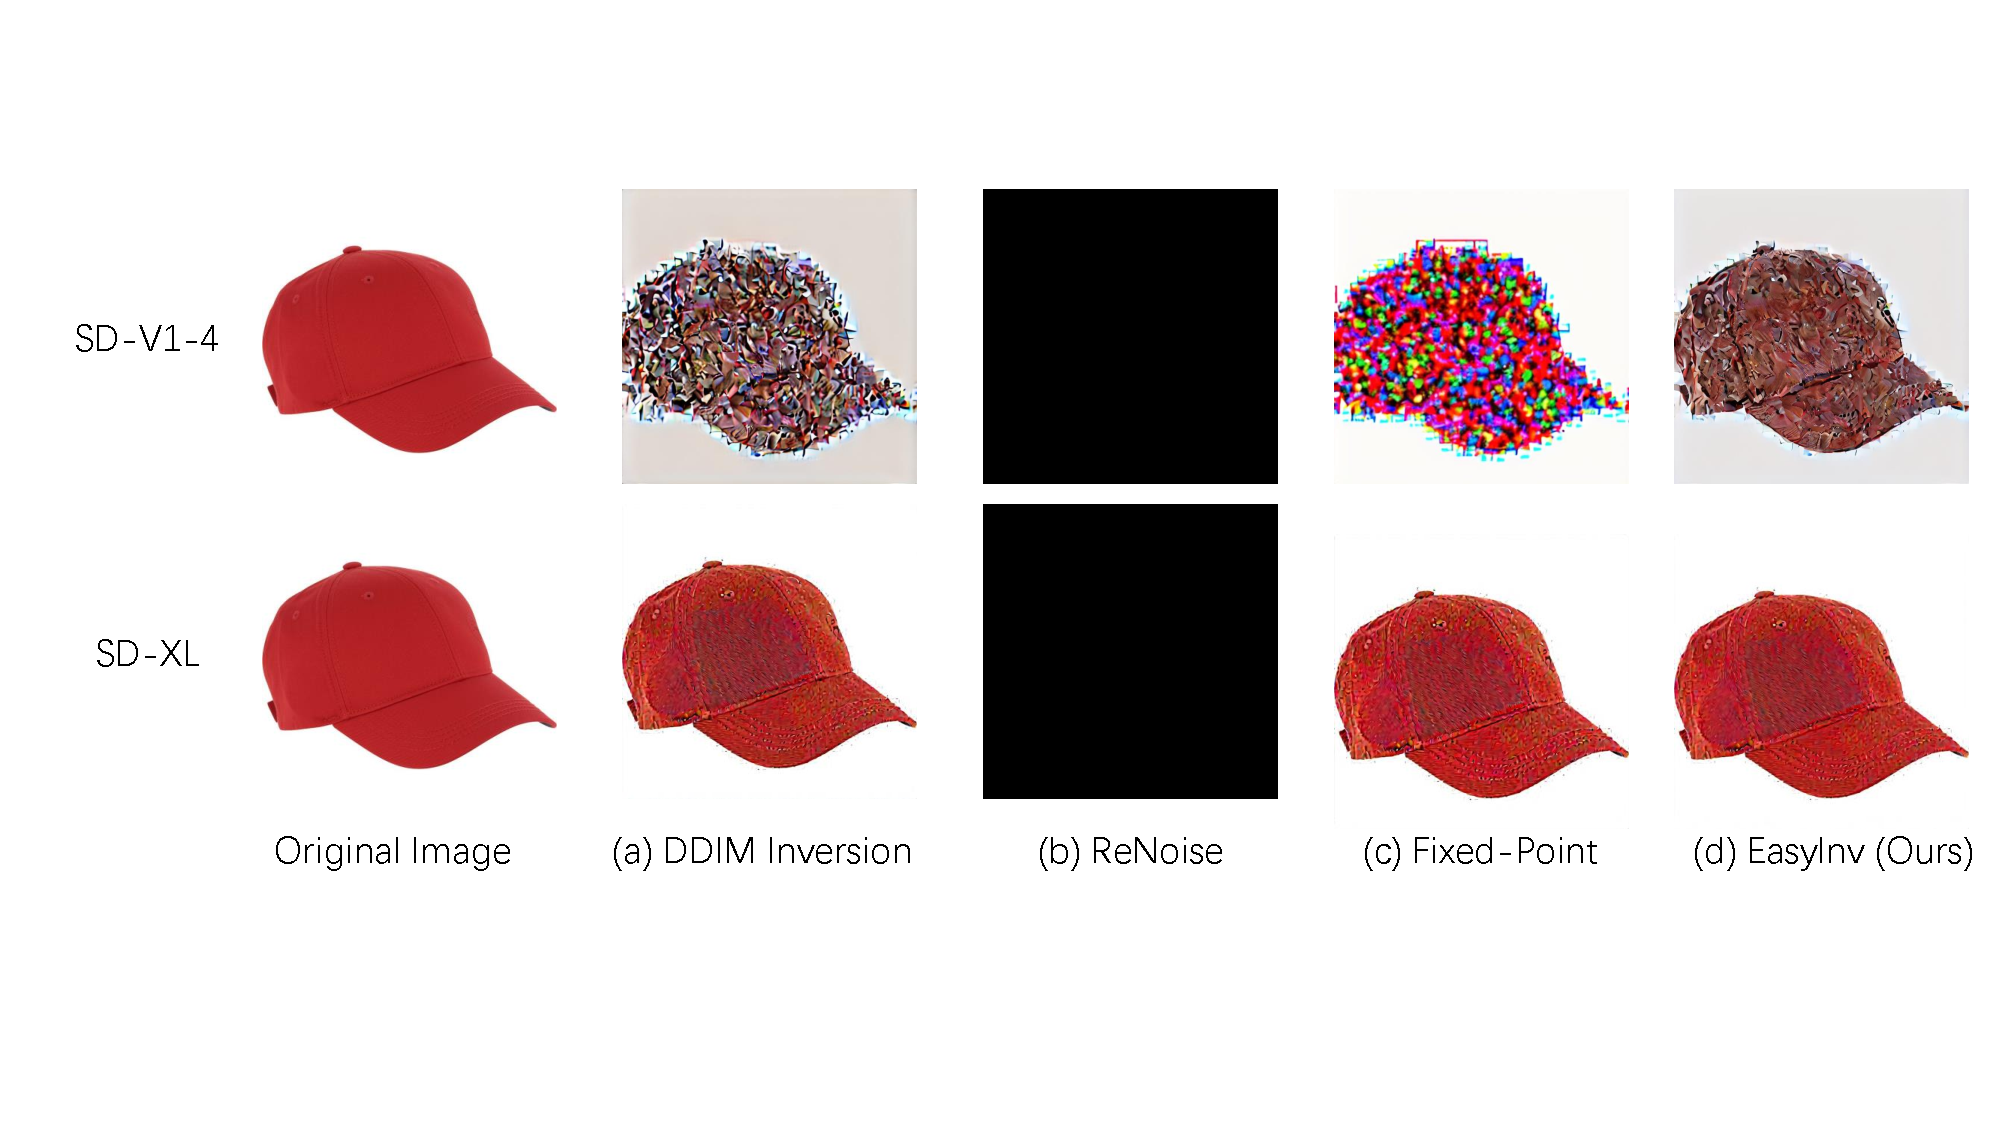
\includegraphics[width=0.98\linewidth]{visual_hat_noise_together_cut.pdf}
  \caption{Visualization of the latent states midway through all denoising steps for various inversion methods. Our EasyInv shows its enhanced convergence by closely approximating the original image.}
  \label{fig_mid_step}
\end{figure}

\section{Related Works}
\label{Re_works}

\textbf{Diffusion Model}.
%
%
In recent years, there has been significant progress in the field of generative models, with diffusion models emerging as a particularly popular approach.
%
The seminal denoising diffusion probabilistic models (DDPM)~\cite{ho2020denoising} introduced a practical framework for image generation based on the diffusion process.
%
This method stands out from its predecessors, such as generative adversarial networks (GANs), due to its iterative nature.
%
During the data preparation phase, Gaussian noise is incrementally added to a real image until it transitions into a state that is indistinguishable from raw Gaussian noise.
%
Subsequently, a model can be trained to predict the noise added at each step, enabling users to input any Gaussian noise and obtain a high-quality image as a result.
%
Ho \emph{et al}.~\cite{ho2020denoising} provided a robust theoretical foundation for their model, which has facilitated further advancements.
%
Generative process in DDPM is both time-consuming and inherently stochastic due to the random noise introduced at each step. To address these limitations, the denoising diffusion implicit models (DDIM) were developed~\cite{song2020denoising}. 
%
By reformulating DDPM, DDIM has successfully reduced the amount of random noise added at each step. This reformulation results in a more deterministic denoising process. Furthermore, the absence of random noise allows for the aggregation of several denoising steps, thereby significantly reducing the overall computation time required to generate an image.


\textbf{Image Inversion}.
%
%
%
Converting a real image into noise is a pivotal first step in the realm of real image editing using diffusion models.
%
The precision of this process has a profound impact in the final edit, with the critical element being the accurate identification of the noise added at each step.
%
Couairon \emph{et al}.~\cite{couairon2023diffedit} ingeniously swapped the roles of independent and implicit variables within the denoising function of the DDIM model, enabling it to predict the noise that should be introduced to the current latents.
%
However, it is essential to recognize that the denoising step in a diffusion model is inherently an approximation, and when this approximation is utilized inversely, discrepancies between the model's output and the actual noise value are likely to be exacerbated.
%
To address this issue, ReNoise \cite{garibi2024renoise} iterates through each noising step multiple times. For each inversion step, they employ an iterative approach to add and subsequently reduce noise, with the noise reduced in the final iteration being carried forward to the subsequent iteration.
%
Pan \emph{et al.}~\cite{pan2023effective} offered a theoretical underpinning to the ReNoise method. Iterative optimization from ReNoise is classified under the umbrella of fixed-point iteration methods. Building upon Anderson's seminal work~\cite{anderson1965iterative}, Pan \emph{et al}. have advanced the field by proposing their novel method for optimizing noise during the inversion process. 


\section{Methodology}
\label{methods}

\subsection{Preliminaries}

\subsubsection{DDIM Inversion}
\label{sec:ddim_inv}

Let \(\mathbf{z}_T\) denote a noise tensor with \(\mathbf{z}_T \sim \mathcal{I}(0, \mathbf{I})\). The DDIM~\cite{couairon2023diffedit} leverages a pre-trained neural network \(\varepsilon_{\theta}\) to perform \(T\) denoising diffusion steps. Each step aims to estimate the underlying noise and subsequently restore a less noisy version of the tensor, \(\mathbf{z}_{t-1}\), from its noisy counterpart \(\mathbf{z}_t\) as:
\begin{small}
\begin{equation}
\label{denoising process}
    \mathbf{z}_{t-1} = \sqrt{\frac{\alpha_{t-1}}{\alpha_t}}\mathbf{z}_t + \Bigg(\sqrt{\frac{1}{\alpha_{t-1}} - 1} - \sqrt{\frac{1}{\alpha_t} - 1} \Bigg)\cdot \varepsilon_{\theta}\big(\mathbf{z}_t,t,\tau_{\theta}(y)\big),
\end{equation}
\end{small}
where \( t = T \rightarrow 1\), and \( \{\alpha_t\}_{t=1}^T \) constitutes a prescribed variances set that guides the diffusion process. Furthermore, \( \tau_{\theta} \) serves as an intermediate representation that encapsulates the textual condition \( y \).  For the convenience of following sections, we denote:
\begin{equation}\label{eq:noise}
  d(\mathbf{z}_t) = \varepsilon_{\theta}\big(\mathbf{z}_t,t,\tau_{\theta}(y)\big).   
\end{equation}



Re-evaluating Eq.\,(\ref{denoising process}), we derive DDIM Inversion process~\cite{couairon2023diffedit} as presented in Eq.(\ref{DDIM-inv}). In this reformulation, we relocate an approximate $\mathbf{z}^*_t$ to the left-hand side, resulting in the following expression:
\begin{small}
\begin{equation}
\label{DDIM-inv}
\begin{split}
\mathbf{z}^*_t &= g\left(\varepsilon_{\theta}\big(\mathbf{z}^*_{t-1},t-1,\tau_{\theta}(y)\big)\right) \\&= \sqrt{\frac{\alpha_{t}}{\alpha_{t-1}}}\mathbf{z}^*_{t-1} -\\& \sqrt{\frac{\alpha_{t}}{\alpha_{t-1}}}\Bigg(\sqrt{\frac{1}{\alpha_{t-1}} - 1} - \sqrt{\frac{1}{\alpha_t} - 1} \Bigg) \cdot \varepsilon_{\theta}\big(\mathbf{z}^*_{t-1},t-1,\tau_{\theta}(y)\big),
\end{split}
\end{equation}
\end{small}

\textbf{Review}. Given an image \(\mathbf{I}^*\), after encoding it into the latent \(\mathbf{z}^*_0\), we initiate \(T\) inversion steps using Eq.\,(\ref{DDIM-inv}) to obtain the noise \(\mathbf{z}^*_T\). Starting with \(\mathbf{z}_T = \mathbf{z}^*_T\), we proceed with a denoising process in Eq.\,(\ref{denoising process}) to infer an approximate reconstruction \(\mathbf{z}_0\) that resembles the original latent  \(\mathbf{z}^*_0\). The primary source of error in this reconstruction arises from the difference between the noise predicted during the inversion process \(\varepsilon_{\theta}\big(\mathbf{z}^*_{t-1}, t-1, \tau_{\theta}(y)\big)\) and the noise expected in the sampling process, \(\varepsilon_{\theta}\big(\mathbf{z}_t, t, \tau_{\theta}(y)\big)\), denoted as \(\varepsilon_t\), at each iterative step. This discrepancy originates from an imprecise approximation of the time step from \(t\) to \(t-1\). Therefore, reducing the discrepancy between the predicted noises at each step is crucial for achieving an accurate reconstruction, which is essential for the success of subsequent image editing tasks. For simplicity in the following expressions, we define:
%
\begin{equation}
    \varepsilon_{t}^* = \varepsilon_{\theta}\big(\mathbf{z}^*_{t-1},t-1,\tau_{\theta}(y)\big), \qquad \varepsilon_t = \varepsilon_{\theta}\big(\mathbf{z}_t,t,\tau_{\theta}(y)\big).
\end{equation}





\subsection{Fixed-Point Iteration}
\label{sec:motivation}
The vanilla DDIM Inversion method, as discussed, involves an approximation that is not entirely precise for \(\varepsilon_t^*\). To address this, researchers have sought to refine a more accurate approximation of \(\varepsilon_t^*\), thereby ensuring that the desired conditions are optimally met. This refinement process aims to enhance the precision of the method, leading to more reliable results in the context of the application:
\begin{equation}\label{eq:goal}
    \varepsilon_t^* = \varepsilon_t.
\end{equation}


For clarity, let's first restate Eq.\,(\ref{DDIM-inv}) as follows:
\begin{equation}\label{eq:forward}
\mathbf{z}^*_t = g(\varepsilon_t^*),
\end{equation}
which represents the introduction of adding noise to the latent state $\mathbf{z}^*_{t-1}$. Under the assumption of Eq. (\ref{eq:goal}), it should be the case that:
\begin{equation}\label{eq:condition}
\mathbf{z}_t = \mathbf{z}_t^*.
\end{equation}


Subsequently, by employing the noise estimation function from Eq.\,(\ref{eq:noise}), we obtain:
\begin{equation}\label{eq:two_functions}
d\big(\mathbf{z}_t) = d\big(g(\varepsilon_t^*)\big).
\end{equation}


Given that $d(\mathbf{z}_t)  = \varepsilon_{t}$ and considering Eq.\,(\ref{eq:goal}), we can deduce that:
\begin{equation}
    \varepsilon_{t}^* = d\big(g(\varepsilon_t^*)\big).
\end{equation}



This formulation presents a fixed-point problem, which pertains to a value that remains unchanged under a specific transformation~\cite{bauschke2011fixed}.  In the context of functions, a fixed point is an element that is invariant under the application of the function. In this paper, we seek a $\varepsilon^*_t$ that, when transformed by $g$ and followed by $d$, can map back to itself, signifying an optimal solution as per Eq. (\ref{eq:goal}).


Fixed-point iteration is a computational technique designed to identify the fixed points of a function. It functions through an iterative process, as delineated below:
\begin{equation}\label{eq:pratical}
(\varepsilon^*_{t})^n = d\big(g(\varepsilon^*_{t})^{n-1}\big),
\end{equation}
where $n$ denotes the iteration count. This iterative process can be enhanced through acceleration techniques such as Anderson acceleration ~\cite{anderson1965iterative}.
%
However, calculating a complex $\varepsilon^*_{t}$ can be quite onerous. An empirical acceleration method proposed~\cite{pan2023effective} introduces a refinement for $\varepsilon_t^*$ by setting: $\big(\varepsilon^*_{t})^n = \varepsilon_{\theta}(({\mathbf{z}^{*}_{t}})^{n},t-1,\tau_{\theta}(y)\big)$ and $(\varepsilon^*_{t})^{n-1} = \varepsilon_{\theta}\big(({\mathbf{z}^{*}_{t}})^{n-1},t-1,\tau_{\theta}(y)\big)$. They finally reach:
\begin{equation}\label{eq:pan_iter}
({\mathbf{z}^{*}_{t}})^{n+1} = g(0.5 \cdot (\varepsilon^*_{t})^n+0.5 \cdot (\varepsilon^*_{t})^{n-1}),
\end{equation}
%
where the term $0.5 \cdot (\varepsilon^*_{t})^n+0.5 \cdot (\varepsilon^*_{t})^{n-1}$ represents the refinement technique for $\varepsilon^*_{t}$ as suggested by Pan \emph{et al.}. If we were to apply the function $d$ to both sides of Eq.\,(\ref{eq:pan_iter}), it would align perfectly with the form of Eq.\,(\ref{eq:pratical}). Their experiments have demonstrated that this approach is more effective than both Anderson's method ~\cite{anderson1965iterative} and other techniques in inversion tasks.



Despite the progress made, this paper acknowledges inherent limitations in the practical implementation of the inversion technique:
%
(1) Inversion Efficiency: While the method outlined in Eq.\,(\ref{eq:pan_iter}) has shown improvements over traditional fixed-point iteration, it still relies on iterative optimization. The need for multiple forward passes through the diffusion model is computationally demanding and can result in inefficiencies in downstream applications.
%
(2) Inversion Performance: The theoretical improvements presented assume that \(\varepsilon^*_t = \varepsilon_t\). However, iterative optimization does not guarantee the exact fulfillment of Equation (\ref{eq:condition}) for every time step \( t \). Therefore, while the method may theoretically offer superior performance, cumulative errors can sometimes lead to practical outcomes that are less satisfactory than those achieved with the standard DDIM Inversion method, as shown in Figure\,\ref{fig_inver}.



\subsection{EasyInv}
\label{sec:ours}

To facilitate our subsequent analysis, we introduce the notation $\bar\alpha_{t}$ to represent $\sqrt{\frac{\alpha_{t}}{\alpha_{t-1}}}$ and $\bar\beta_{t}$ to denote $\sqrt{\frac{\alpha_{t}}{\alpha_{t-1}}}\Big(\sqrt{\frac{1}{\alpha_{t-1}} - 1} - \sqrt{\frac{1}{\alpha_t} - 1} \Big)$. With these notations, we can reframe Eq.\,(\ref{DDIM-inv}) as follow:
\begin{equation}\label{eq:x_t}
\mathbf{z}^*_{t}=\bar\alpha_{t}\mathbf{z}^*_{t-1} + \bar\beta_{t}\varepsilon^*_{t},
\end{equation}



Similarly, we can express the form of $\mathbf{z}^*_{t-1}$ as:
\begin{equation}\label{eq:x_t-1}
\mathbf{z}^*_{t-1}=\bar\alpha_{t-1}\mathbf{z}^*_{t-2} + \bar\beta_{t-1}\varepsilon^*_{t-1},
\end{equation}


By combining these two formulas, we derive:
\begin{equation}\label{eq:reformed_x_t}
\mathbf{z}^*_{t}=\bar\alpha_{t}\bar\alpha_{t-1}\mathbf{z}^*_{t-2} + \bar\alpha_{t}\bar\beta_{t-1}\varepsilon^*_{t-1} + \bar\beta_{t}\varepsilon^*_{t}.
\end{equation}



This can be further generalized to:
\begin{equation}\label{eq:ordinary_zt}
\mathbf{z}^*_{t} = (\prod_{i=1}^{t}\bar\alpha_i)\mathbf{z}^*_{0} + \sum_{i=1}^{t}(\bar\beta_i\prod_{j = i+1}^{t}\bar\alpha_j)\varepsilon^*_i.
\end{equation}



From Eq.\,(\ref{eq:ordinary_zt}), it is evident that $\mathbf{z}^*_{t}$ is a weighted sum of $\mathbf{z}_{0}$ and a series of noise terms $\varepsilon^*_i$. The denoising process of Eq.\,(\ref{denoising process}) aims to iteratively reduce the impact of these noise terms. In prior research, the crux of inversion is to introduce the appropriate noise $\varepsilon^*_i$ at each step to identify a suitable $\mathbf{z}^*_{t}$. This allows the model to obtain $\mathbf{z}_{0}$ as the final output after the denoising process. However, iteratively updating $\varepsilon^*_i$ can be time-consuming, and when the model lacks high precision,  achieving satisfactory results within a reasonable number of iterations may be challenging.


To address this, we propose an alternative perspective. During inversion, rather than searching for better noise, we aggregate the latent state from the last time step $\mathbf{z}^*_{\bar{t}-1}$ with the current latent state $\mathbf{z}^*_{\bar{t}}$ at specific time steps $\bar{t}$, as illustrated in the following formula:
\begin{equation}\label{eq:inject}
\mathbf{z}^*_{\bar{t}}=\eta  \mathbf{z}^*_{\bar{t}} + (1-\eta)  \mathbf{z}^*_{{\bar{t}-1}},
\end{equation}
where $\eta$ is a trade-off parameter, typically set to $\eta \geq 0.7$. The selection of $\bar{t}$ will be discussed in Sec.\,\ref{sec:quantitative}. This approach effectively increases the weight $\mathbf{z}_{0}$ in $\mathbf{z}^*_{\bar{t}}$, since:
\begin{equation}\label{eq:prove}
\begin{split}
\mathbf{z}^*_{{\bar{t}-1}} - \mathbf{z}^*_{\bar{t}} = (\prod_{i=1}^{\bar{t}-1}\bar\alpha_i)(1 - \bar\alpha_{\bar{t}})\mathbf{z}_{0} \\+ (1 - \bar\alpha_{\bar{t}})\sum_{i=1}^{\bar{t}-1}(\bar\beta_i\prod_{j = i+1}^{\bar{t}-1}\bar\alpha_j)\varepsilon^*_i + (-\bar\beta_{t})\varepsilon^*_{\bar{t}}
\end{split}
\end{equation}


Given that $0 < \bar\alpha_i < 1$, for $ i = 0 \rightarrow \bar{t}$, it follows that $(\prod_{i=0}^{\bar{t}-1}\bar\alpha_i)(1 - \bar\alpha_{\bar{t}}) > 0$. Consequently, in comparison to \(\mathbf{z}^*_{\bar{t}}\), \(\mathbf{z}^*_{\bar{t}-1}\) carries a higher proportion of \(\mathbf{z}_0\) and is, therefore, less susceptible to the influence of noise. Our approach, therefore, accentuates the significance of the initial latent state \(\mathbf{z}_0\), which encapsulates the most comprehensive information regarding the original image, within \(\mathbf{z}^*_{\bar{t}}\).


%One potential risk associated with our method is the possibility of ``over-denoising,'' which results from an emphasis on achieving a cleaner final-step latent state and can occasionally lead to overly smooth image outputs. However, as our experimental results demonstrate, the method's two key advantages substantially outweigh this minor drawback. Firstly, it is capable of producing satisfactory results even with models that underperform when compared to other methods, as detailed in Figure\,\ref{SDV1-4_compare}. Secondly, it enhances inversion efficiency by reverting to the original DDIM Inversion baseline~\cite{couairon2023diffedit}, thus eliminating the need for iterative optimizations. This approach not only streamlines the process but also maintains high-quality outputs, making it a valuable improvement over existing methods.



\begin{table*}[!t]\tabcolsep=0.4cm
\caption{A comparative analysis of quantitative outcomes utilizing the SD-V1-4 model.}
\centering
 \begin{tabular}{c c c c c} 
 \toprule
 & LPIPS ($\downarrow$) & SSIM ($\uparrow$) & PSNR ($\uparrow$) & Time ($\downarrow$) \\ [0.5ex] 
 \midrule
 DDIM Inversion & 0.328  & 0.621 & 29.717 & \textbf{5s}\\
 \hline
 ReNoise & \textbf{0.316} & 0.641 & \textbf{31.025} & 16s\\
 \hline
 Fixed-Point Iteration & 0.373 & 0.563 & 29.107 & 14s\\
 \hline
 EasyInv (Ours) & 0.321 & \textbf{0.646} & 30.189 & \textbf{5s} \\
 \bottomrule
\end{tabular}
\label{quantitative}
\end{table*}


\begin{table*}[!tb]\tabcolsep=0.4cm
\caption{A comparative analysis of half- and full-precision EasyInv utilizing the SD-V1-4.}
\centering
 \begin{tabular}{c c c c c} 
 \toprule
 & LPIPS ($\downarrow$) & SSIM ($\uparrow$) & PSNR ($\uparrow$) & Time ($\downarrow$) \\ [0.5ex] 
 \midrule
 Full Precision & 0.321 & 0.646 & 30.184 & 9s\\
 \hline
 Half Precision & 0.321 & 0.646 & \textbf{30.189} & \textbf{5s} \\
 \bottomrule
\end{tabular}
\label{precision_table}
\end{table*}


\section{Experimentation}
\label{exp}


We compare our EasyInv over the vanilla DDIM Inversion ~\cite{couairon2023diffedit}, ReNoise~\cite{garibi2024renoise}, Pan \emph{et al.}'s method~\cite{pan2023effective} (referred to as Fixed-Point Iteration), using SD V1.4 and SD-XL on one NVIDIA GTX 3090 GPU. 
%


For Fixed-Point Iteration~\cite{pan2023effective}, we re-implemented it using settings from the paper, as the source code is unavailable. We set the data type of all methods to float16 by default to improve efficiency. The inversion and denoising steps \(T = 50\), except for Fixed-Point Iteration, which recommends \(T = 20\). For our EasyInv, we use \(0.85 \cdot T < \bar{t} < 0.95 \cdot T\) and \(\eta = 0.8\) with the SD-XL framework, and \(0.05 \cdot T < \bar{t} < 0.25 \cdot T\) and \(\eta = 0.5\) with SD-V1-4, due to the varying capacities of the two models.



For quantitative comparison, we use three major metrics: LPIPS index~\cite{zhang2018unreasonable}, SSIM~\cite{wang2004image}, and PSNR. The LPIPS index uses a pre-trained VGG16~\cite{simonyan2015very} to compare image pairs. SSIM and PSNR measure image similarity. We also report inference time. We randomly sample 2,298 images from the COCO 2017 test and validation sets~\cite{COCO}. With the well-trained SD-XL model, error accumulation is minimal, making all methods perform similarly. Therefore, we display results using the SD-V1-4 model.



\begin{figure}[!t]
    \centering
    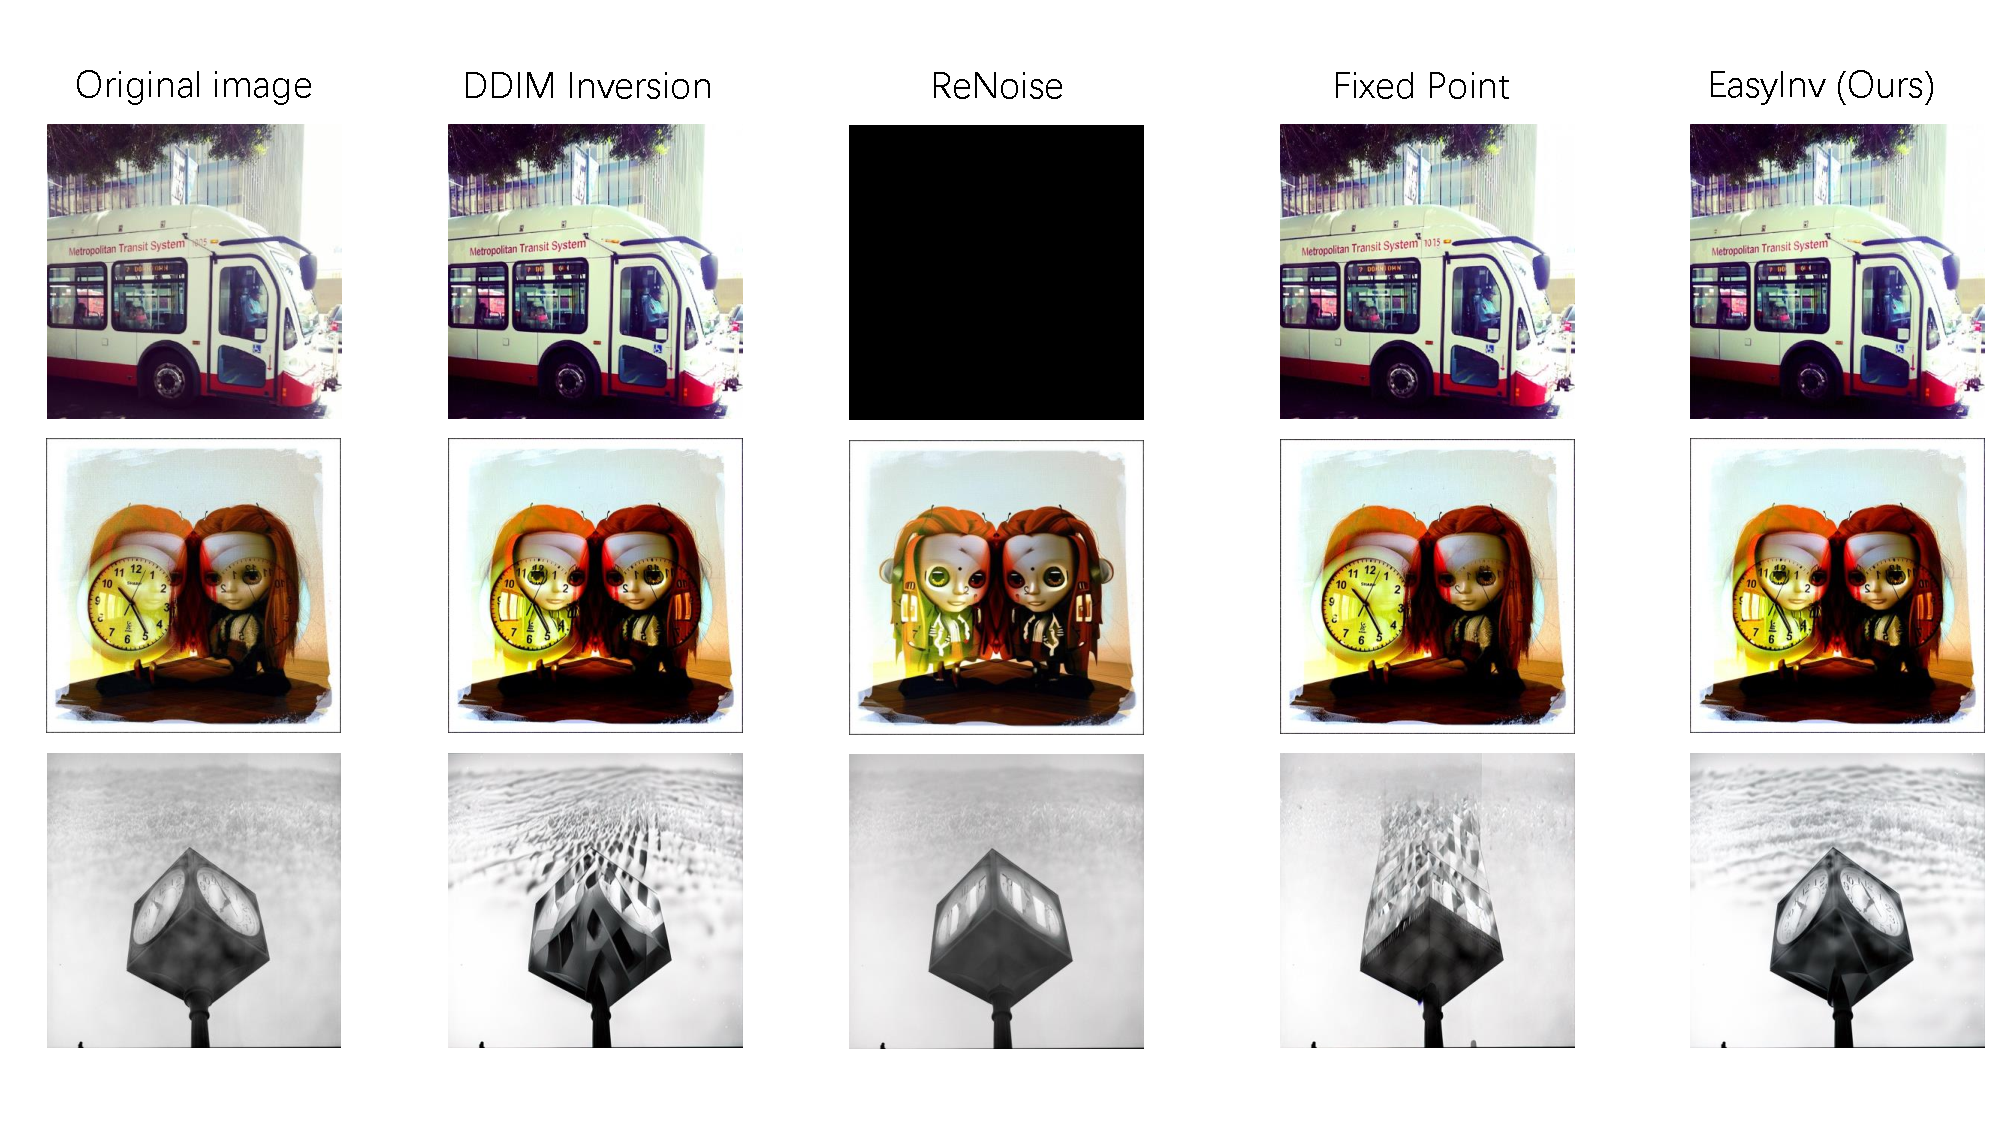
\includegraphics[width=0.98\linewidth]{visual_SDXL.pdf}
    \caption{A visual assessment of various inversion techniques utilizing the SD-XL model.}
    \label{SDXL_compare}
%    \vspace{-0.5cm}
\end{figure}


%
\begin{figure}[!t]
    \centering
    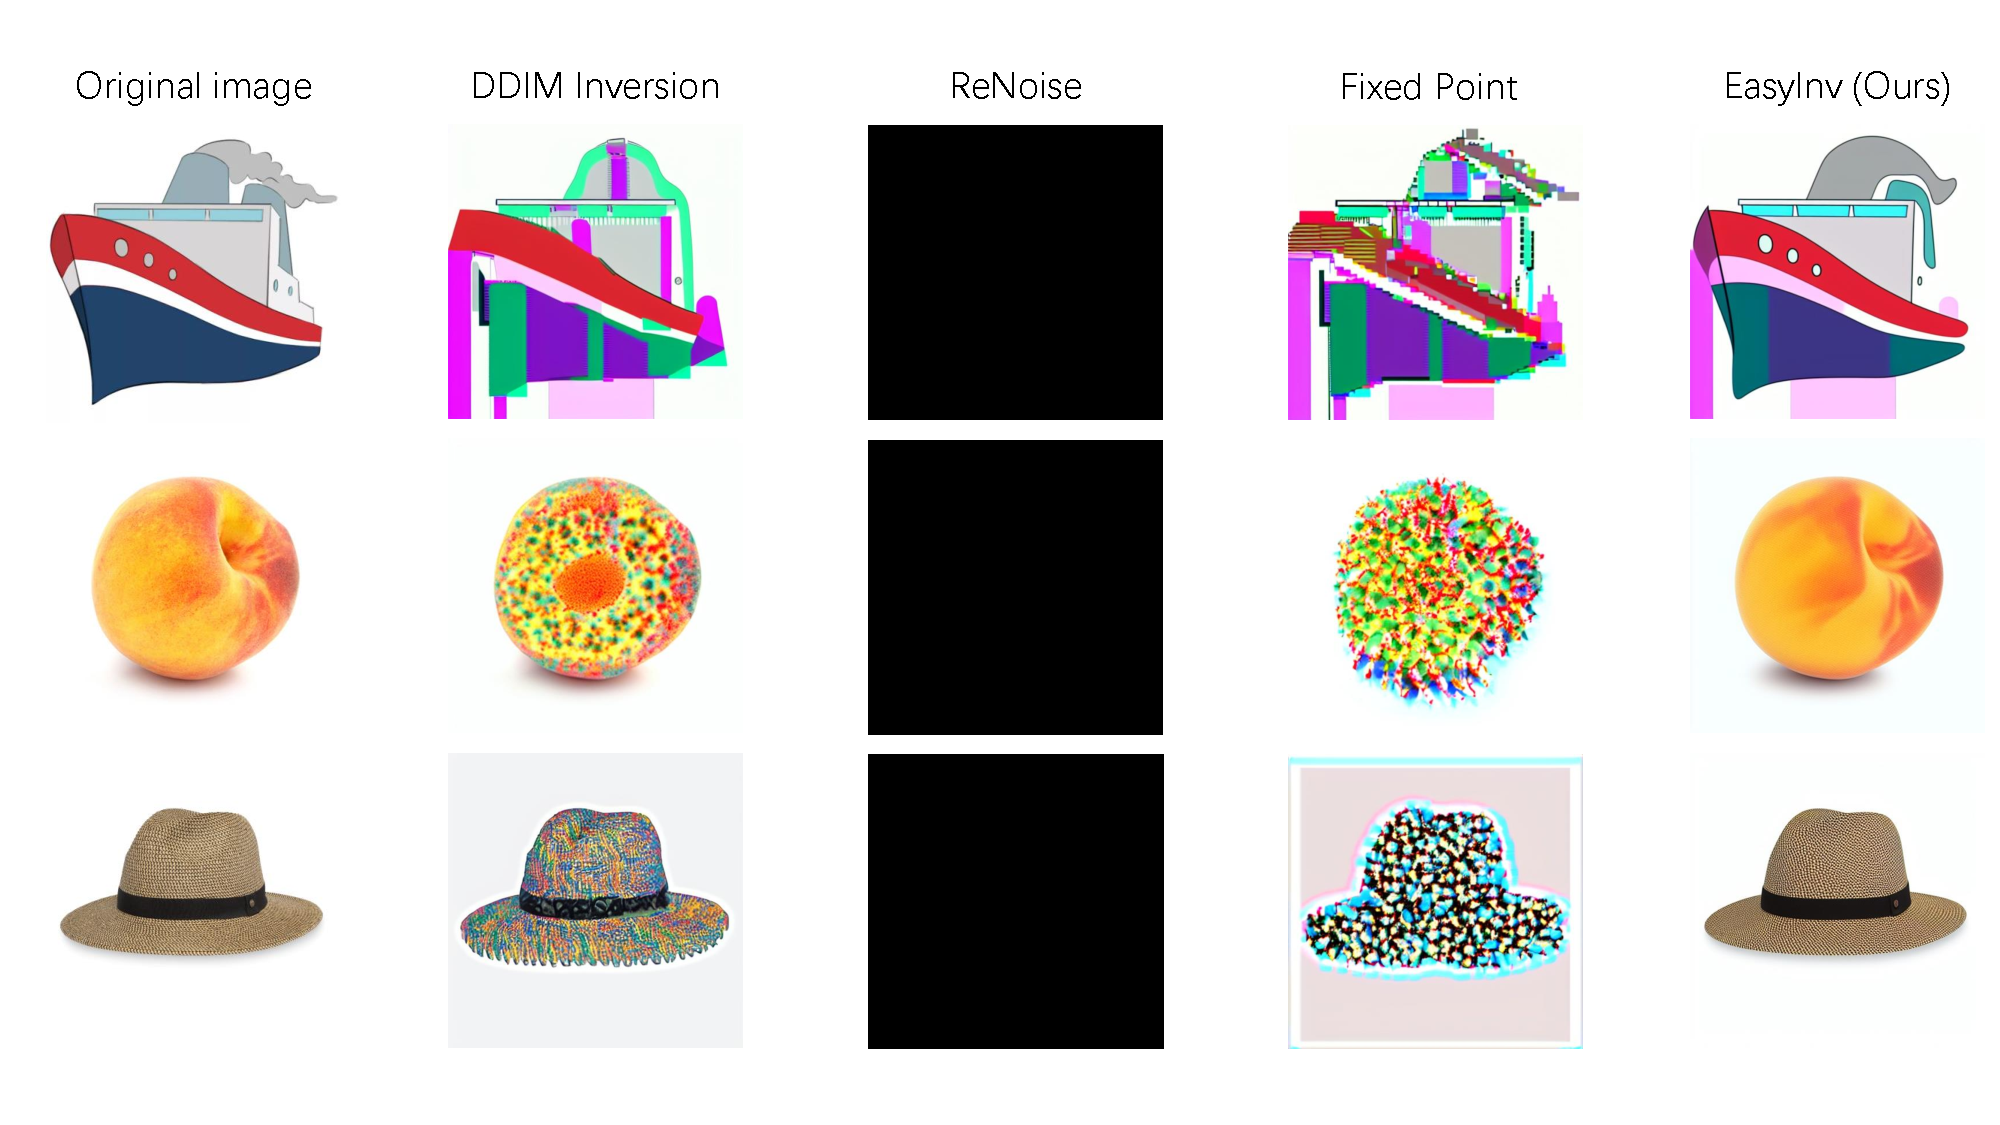
\includegraphics[width=0.98\linewidth]{visual_SDV1-4.pdf}
    \caption{A visual assessment of various inversion techniques utilizing the SD-V1-4 model.}
    \label{SDV1-4_compare}
\end{figure}




\subsection{Quantitative Results}
\label{sec:quantitative}
%
Table\,\ref{quantitative} presents the quantitative results of different methods. EasyInv achieves a competitive LPIPS score of 0.321, better than ReNoise (0.316) and Fixed-Point Iteration (0.373), indicating closer perceptual similarity to the original image. For SSIM, EasyInv achieves the highest score of 0.646, showing superior structural similarity crucial for maintaining image coherence. For PSNR, EasyInv scores 30.189, close to ReNoise's highest score of 31.025, indicating high image fidelity. EasyInv completes the inversion process in the fastest time of 5 seconds, matching DDIM Inversion, and significantly quicker than ReNoise (16 seconds) and Fixed-Point Iteration (14 seconds), highlighting its efficiency without compromising on quality. In summary, EasyInv performs strongly across all metrics, with the highest SSIM score indicating effective preservation of image structure. Its efficient inversion makes it highly suitable for real-world applications where both quality and speed are crucial.


Table\,\ref{precision_table} compares EasyInv's performance in half-precision (float16) and full-precision (float32) formats. Both achieve the same LPIPS score of 0.321, indicating consistent perceptual similarity to the original image. Similarly, both achieve an SSIM score of 0.646, showing preserved structural integrity with high fidelity. For PSNR, half precision slightly outperforms full precision with scores of 30.189 and 30.184. This slight advantage in PSNR for half precision is noteworthy given its well reduced computation time. The most significant difference is observed in the time metric, where half precision completes the inversion process in 5 seconds, approximately 44\% faster than full precision, which takes 9 seconds. This efficiency gain highlights EasyInv's exceptional optimization for half precision, offering faster speeds and reduced resources without compromising output quality.



\begin{figure*}
\centering
\setlength{\tabcolsep}{1pt}
\begin{tabular}
{>{\centering\arraybackslash}m{0.22\linewidth} >{\centering\arraybackslash}m{0.22\linewidth} @{\hspace{0.5cm}} >{\centering\arraybackslash}m{0.22\linewidth} >{\centering\arraybackslash}m{0.22\linewidth}}
    \begin{minipage}{\linewidth}
        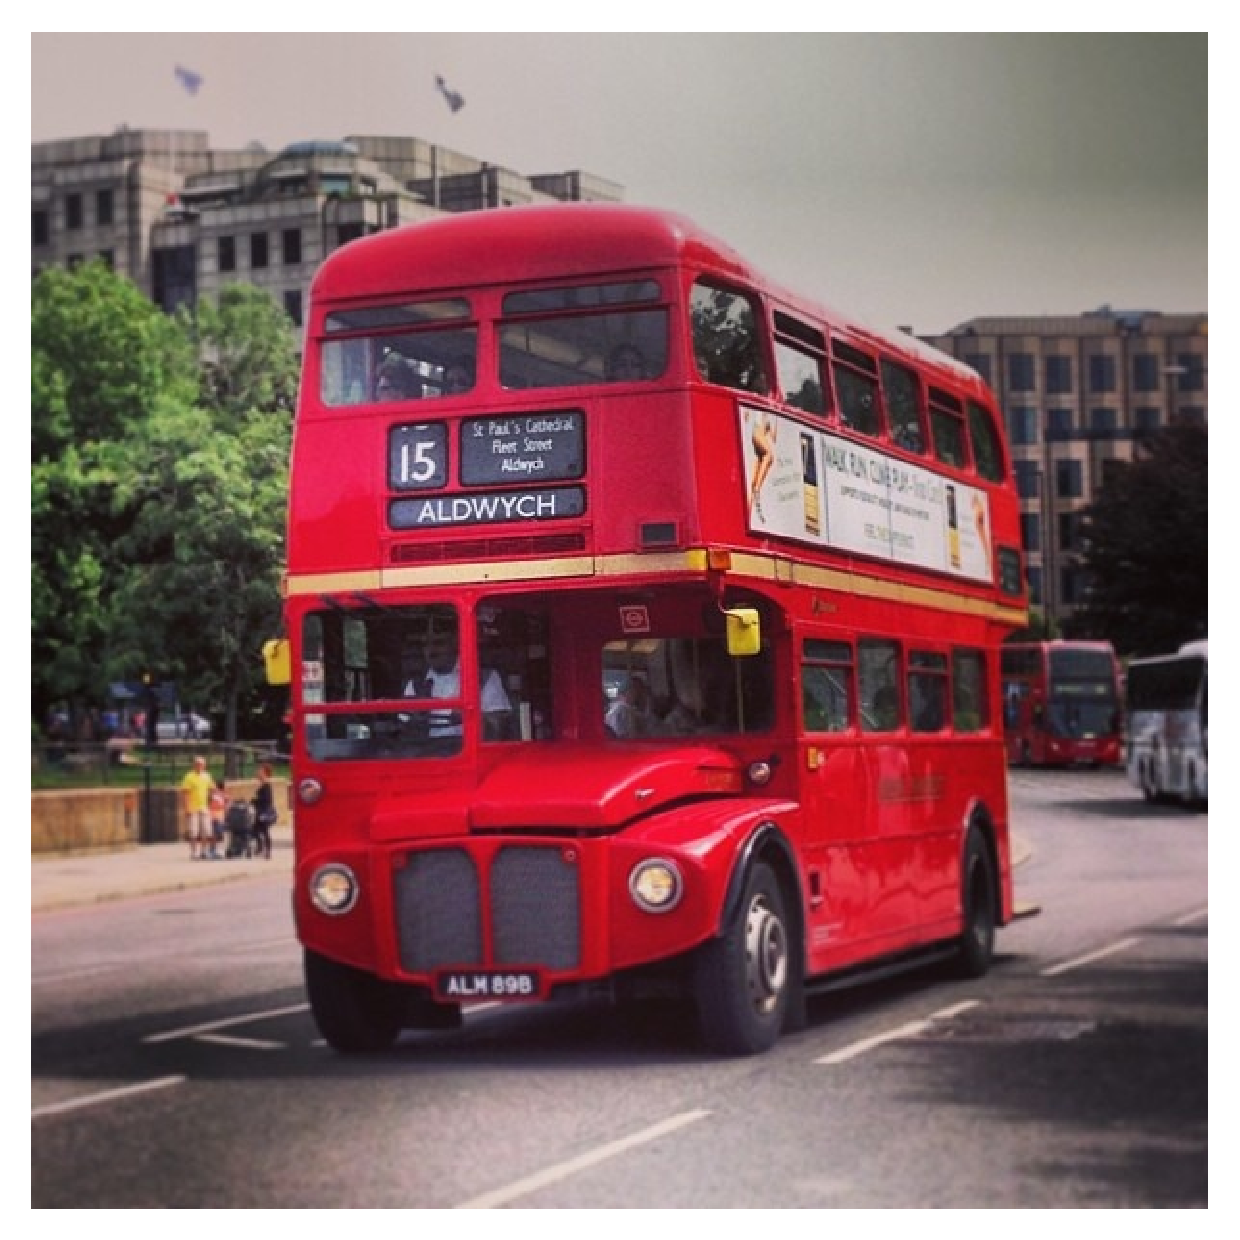
\includegraphics[width=\linewidth]{original_compare/2.pdf}
    \end{minipage} &
    \begin{minipage}{\linewidth}
        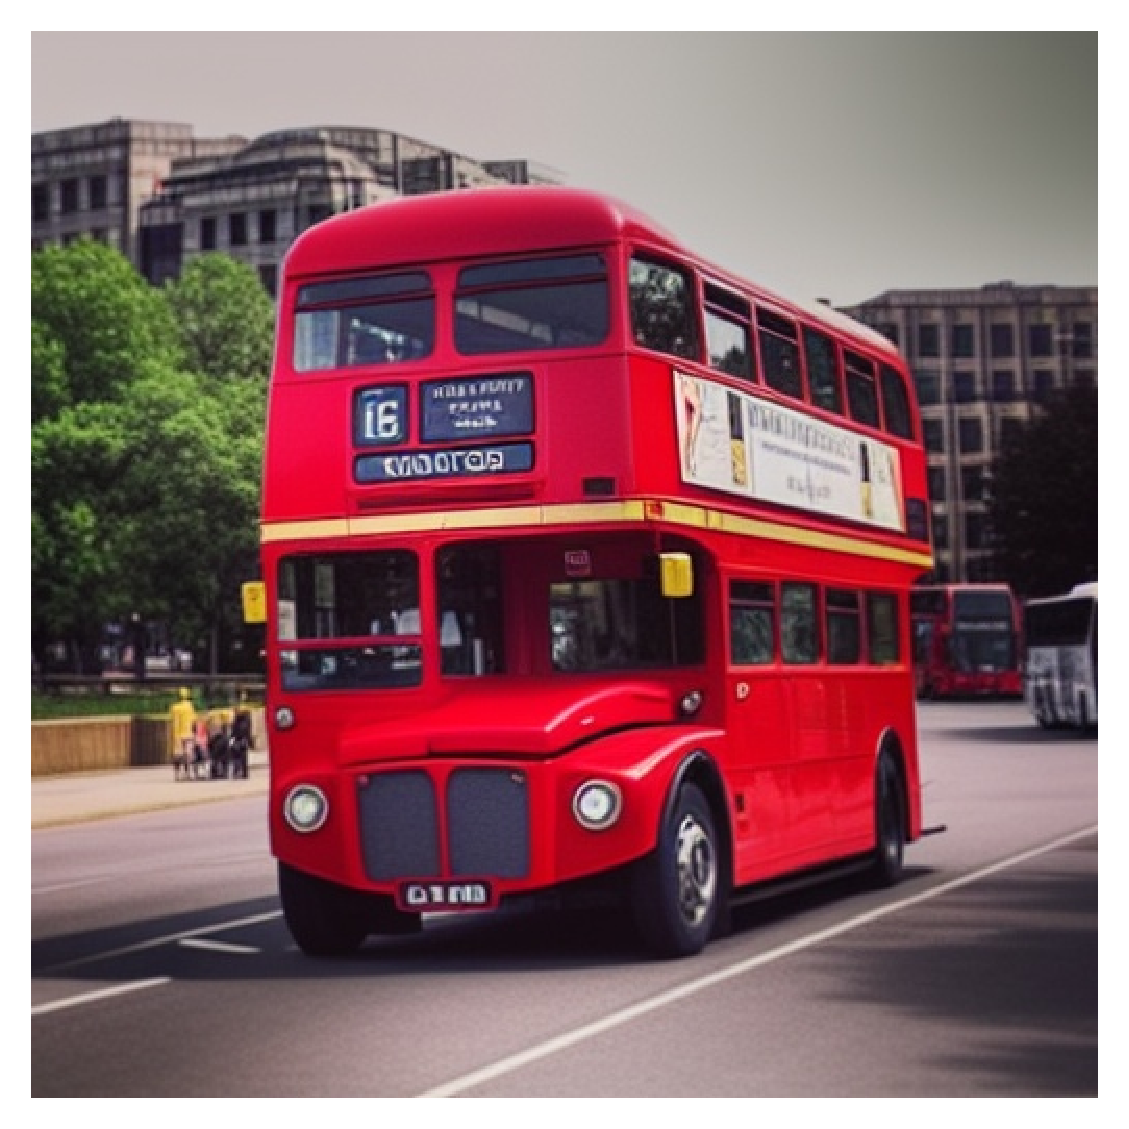
\includegraphics[width=\linewidth]{Ours_compare/2.pdf}
    \end{minipage} &
    \begin{minipage}{\linewidth}
        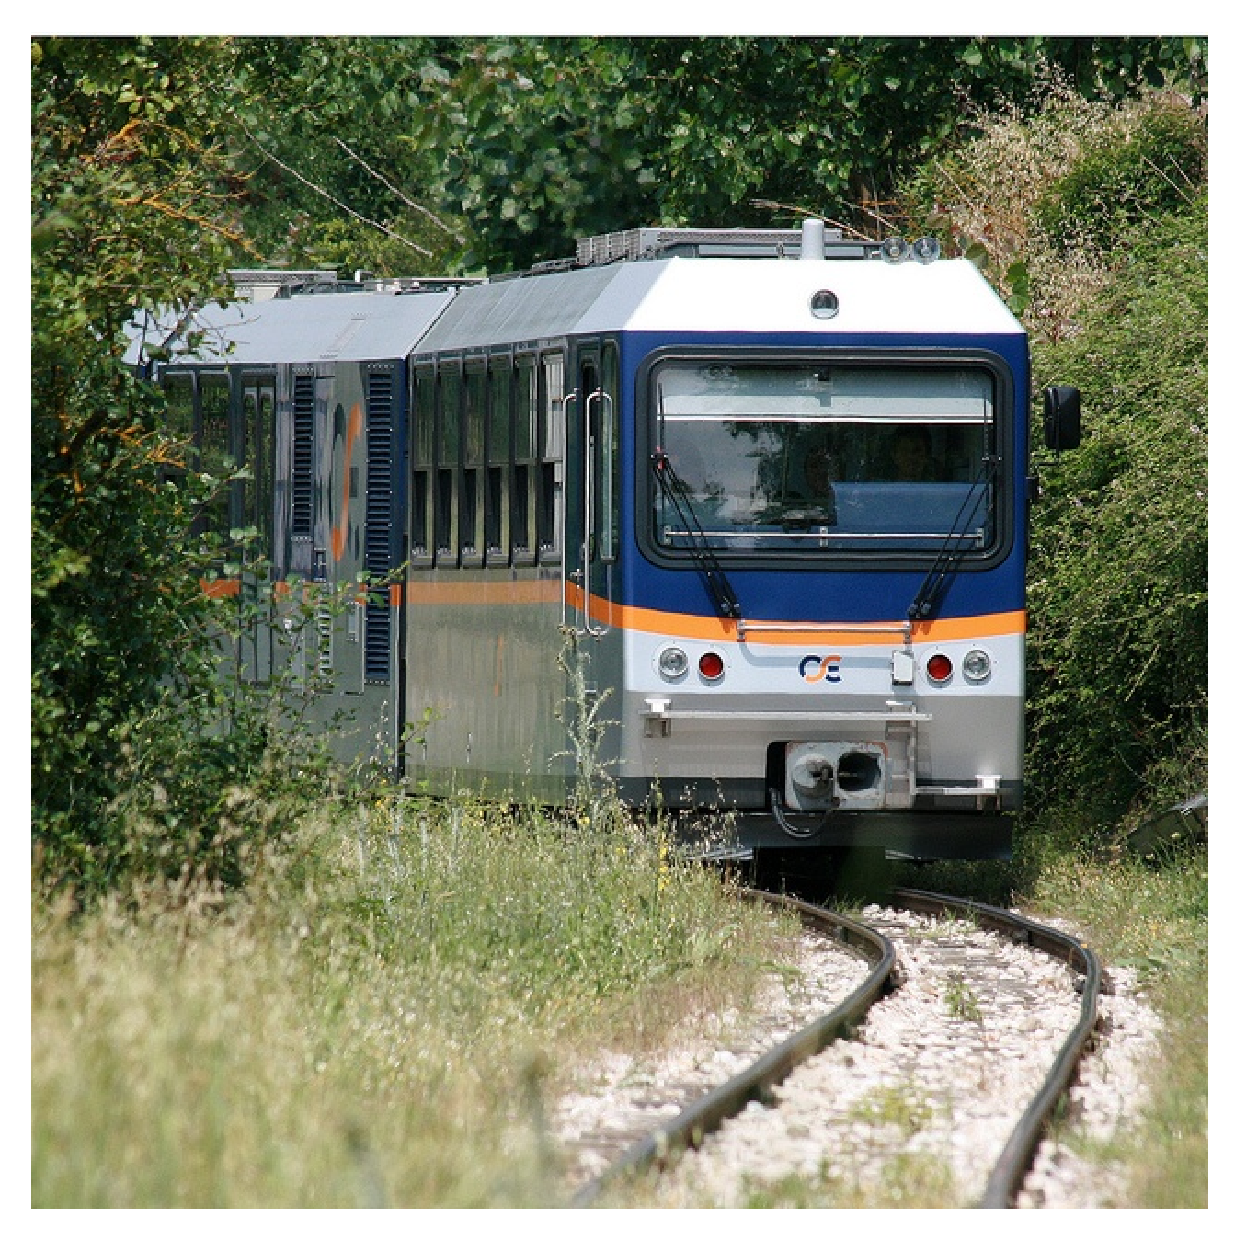
\includegraphics[width=\linewidth]{original_compare/20.pdf}
    \end{minipage} &
    \begin{minipage}{\linewidth}
        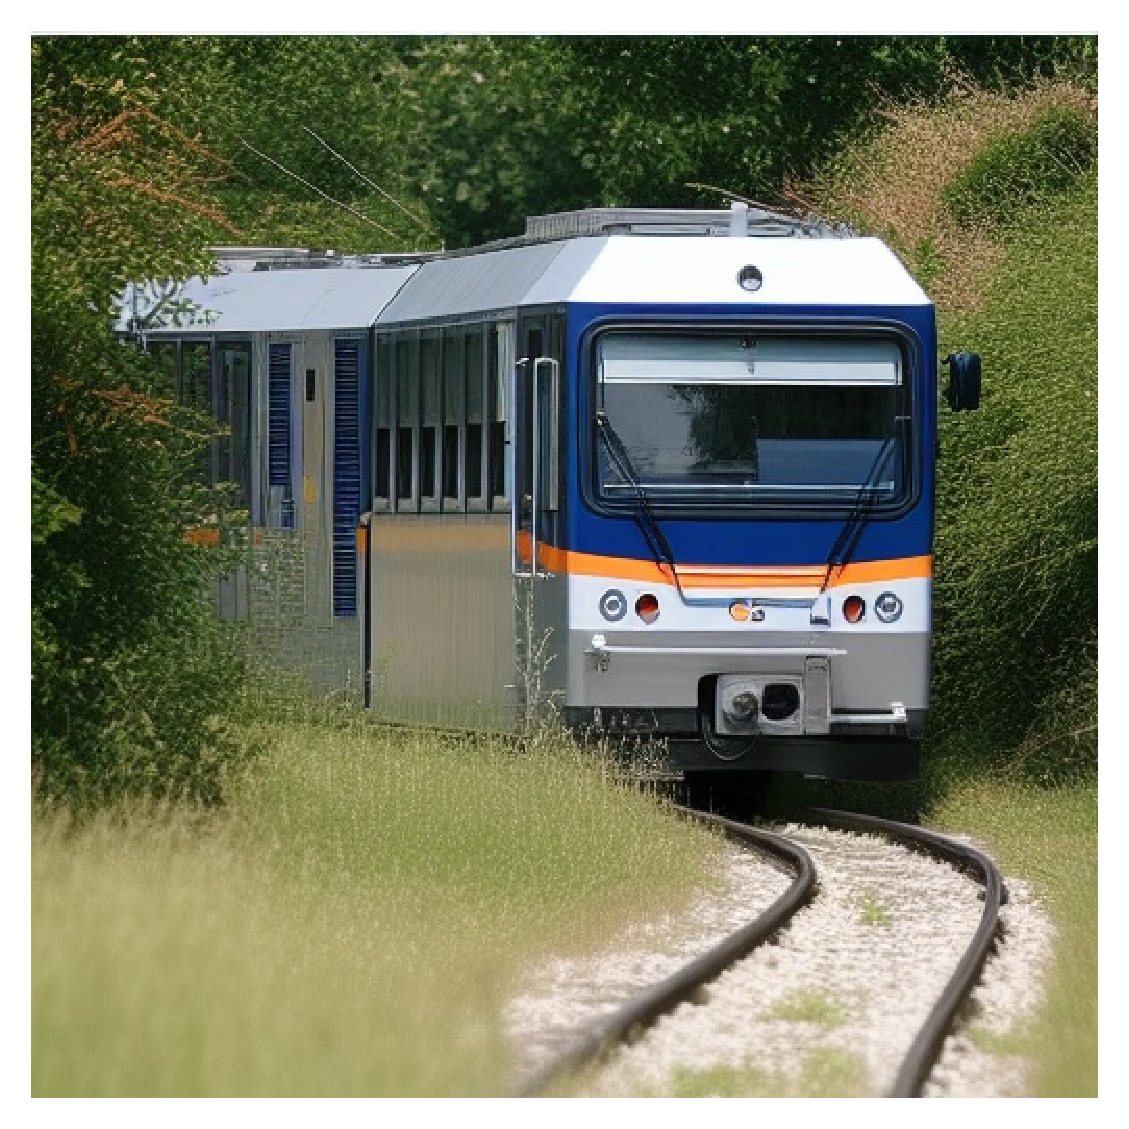
\includegraphics[width=\linewidth]{Ours_compare/20.pdf}
    \end{minipage}
    \\
    \begin{minipage}{\linewidth}
        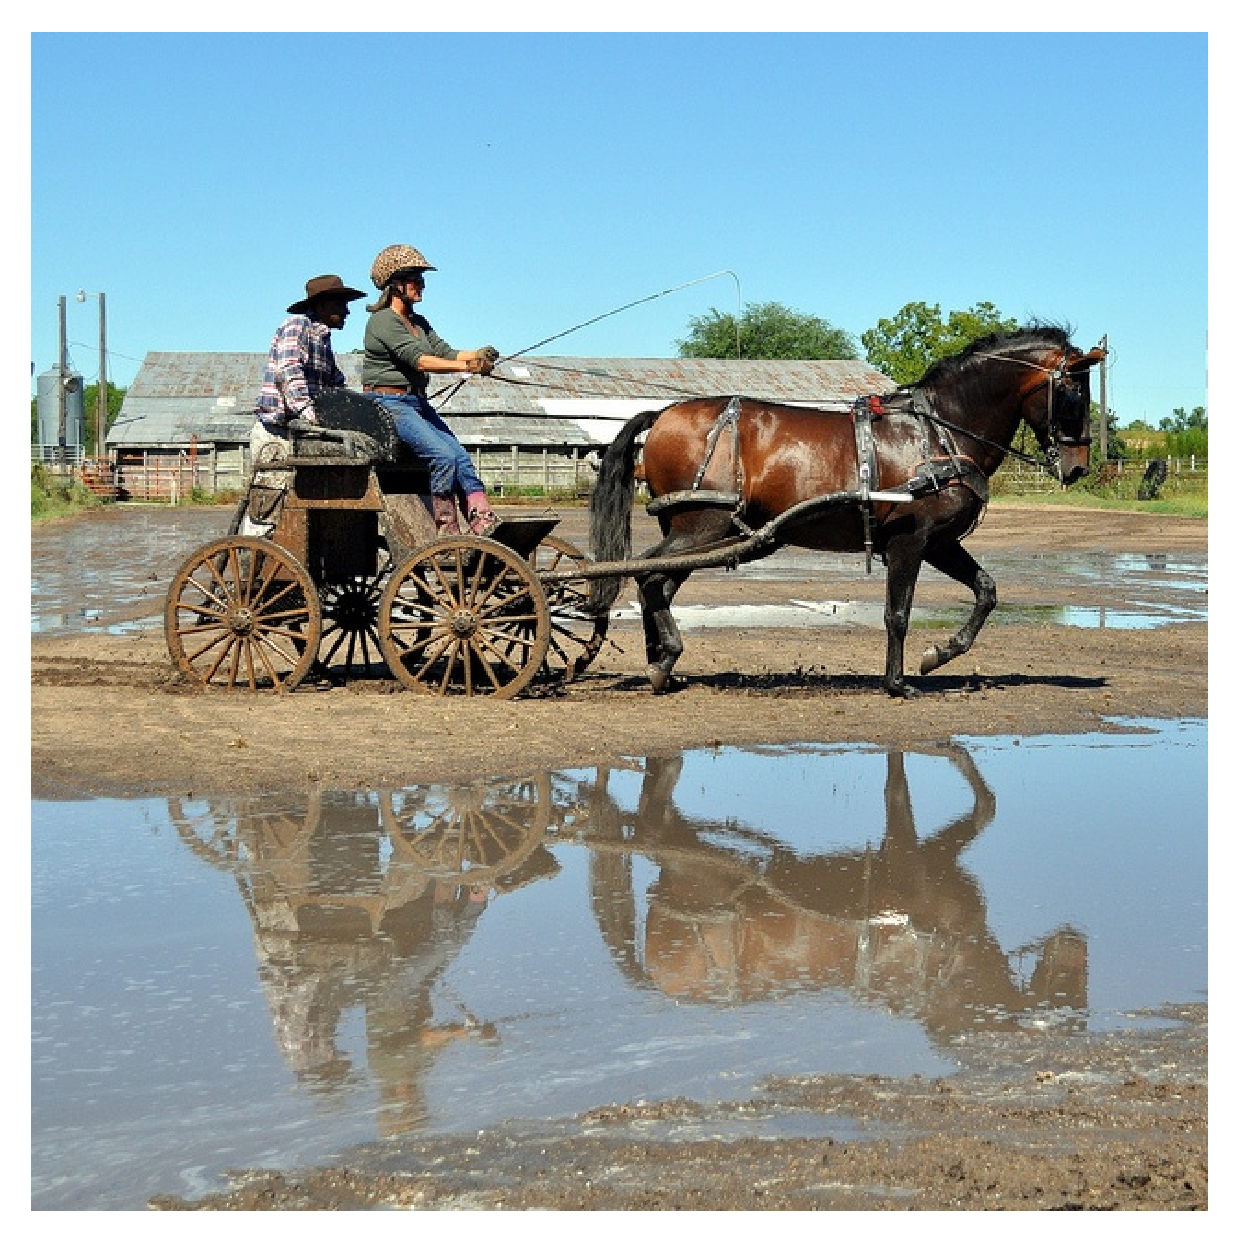
\includegraphics[width=\linewidth]{original_compare/24.pdf}
    \end{minipage} &
    \begin{minipage}{\linewidth}
        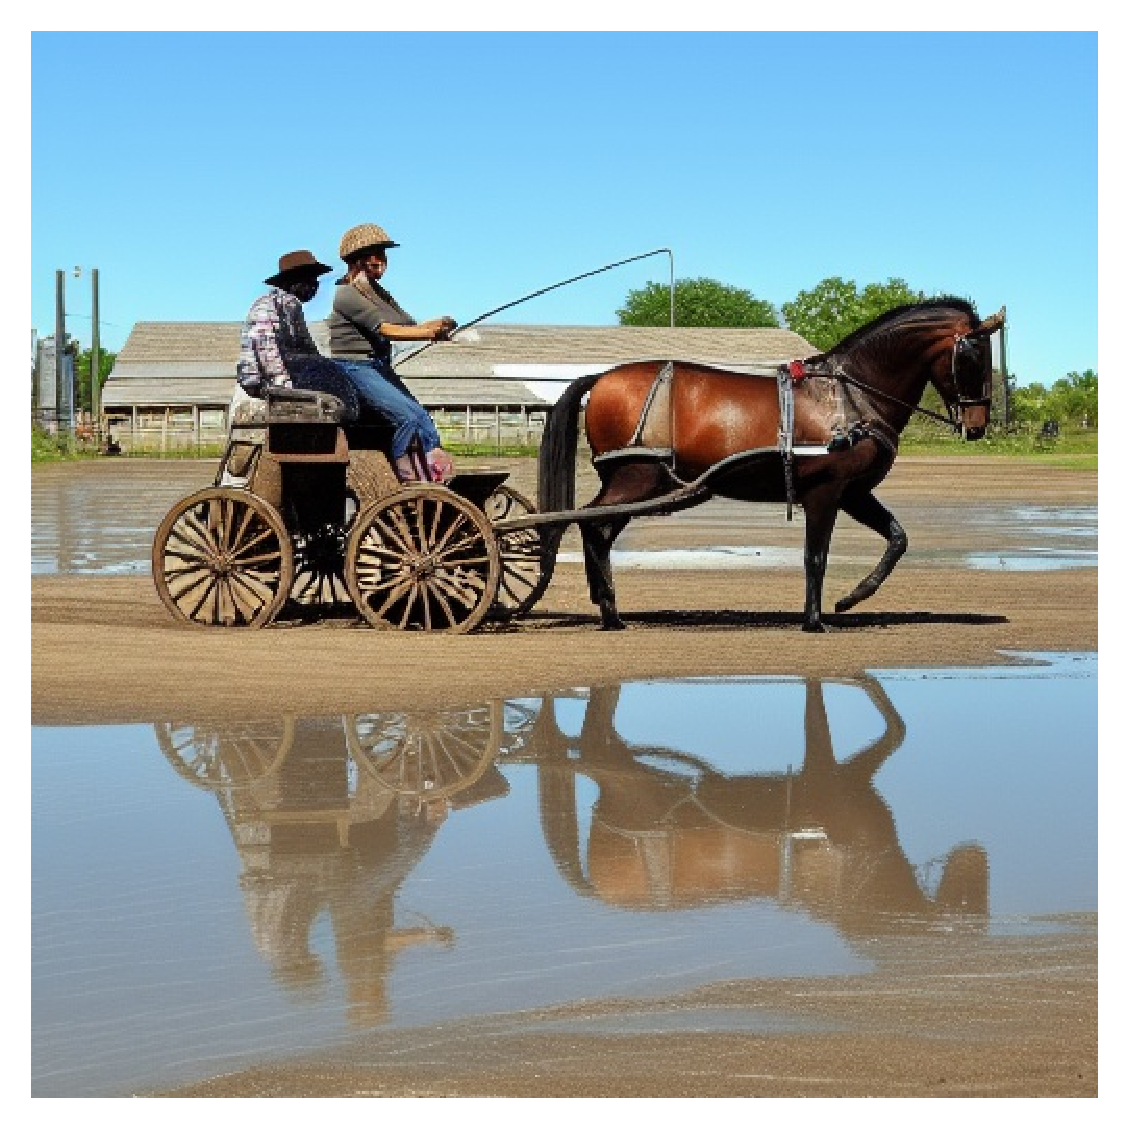
\includegraphics[width=\linewidth]{Ours_compare/24.pdf}
    \end{minipage} &
    \begin{minipage}{\linewidth}
        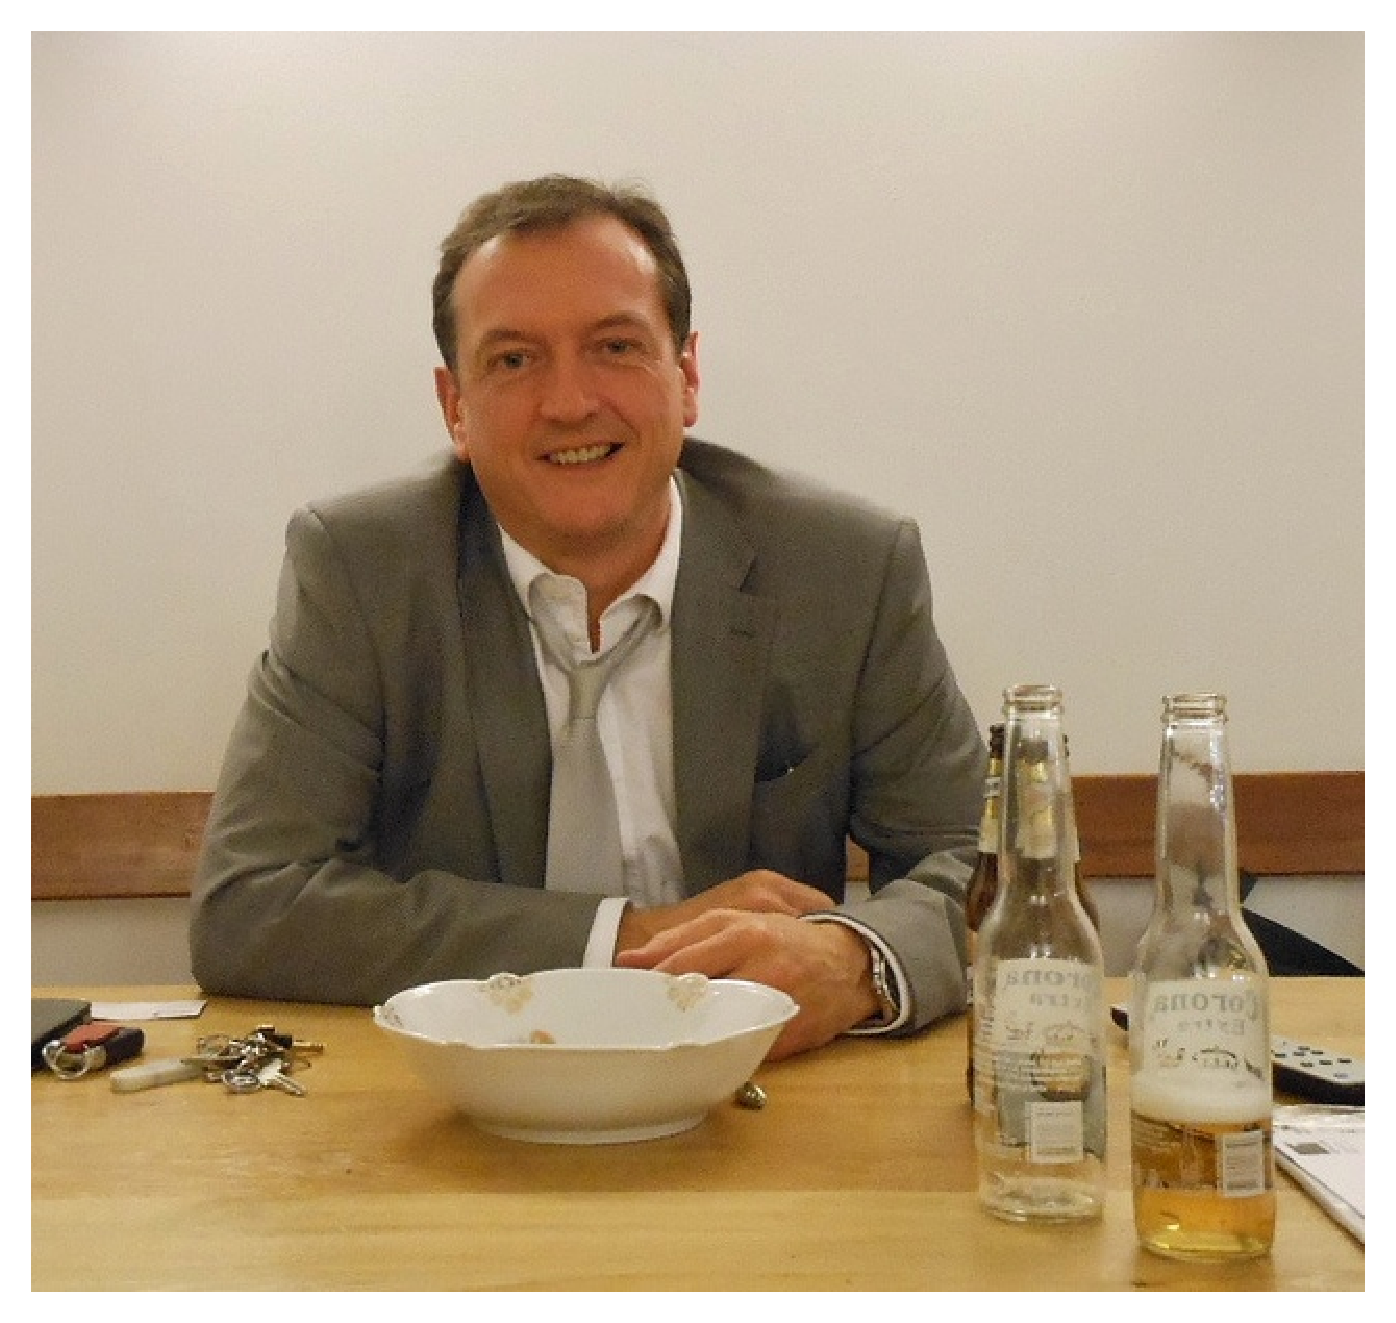
\includegraphics[width=\linewidth]{original_compare/26.pdf}
    \end{minipage} &
    \begin{minipage}{\linewidth}
        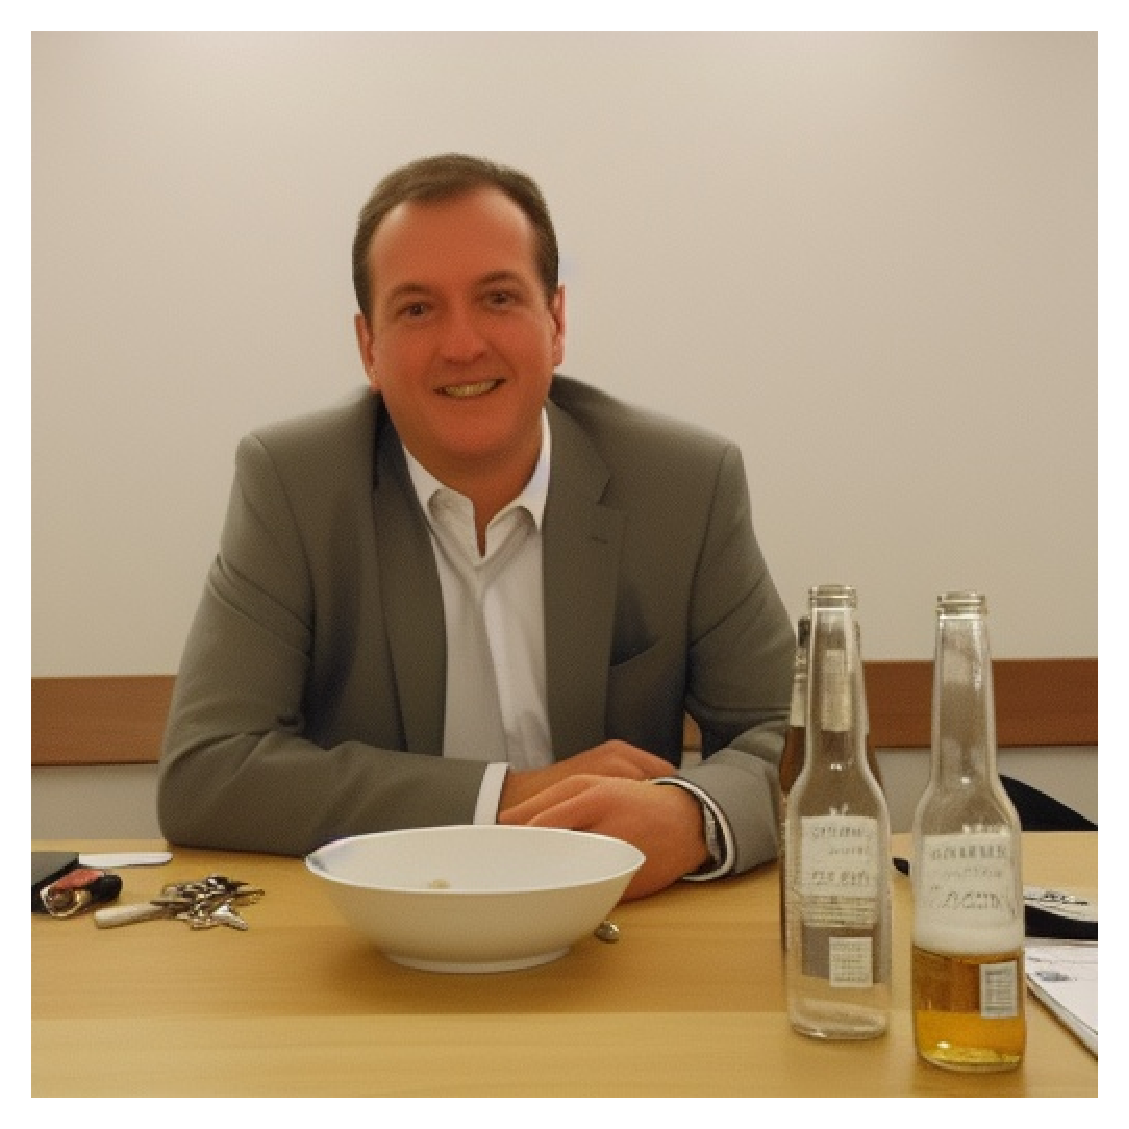
\includegraphics[width=\linewidth]{Ours_compare/26.pdf}
    \end{minipage}
    \\
    \begin{minipage}{\linewidth}
        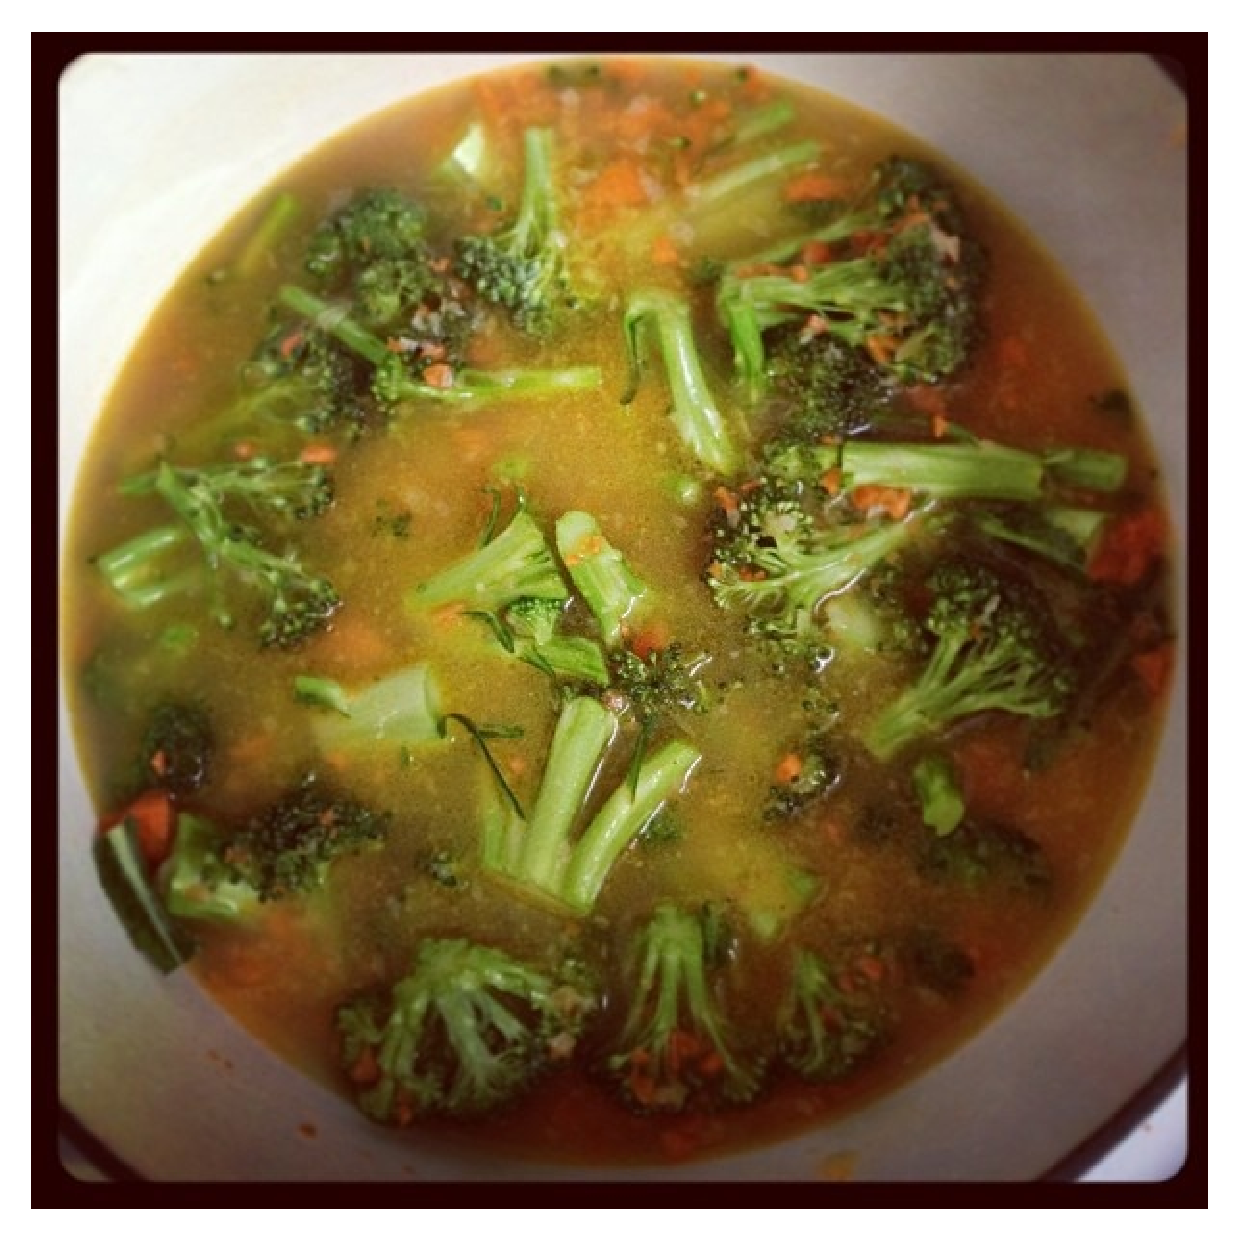
\includegraphics[width=\linewidth]{original_compare/58.pdf}
    \end{minipage} &
    \begin{minipage}{\linewidth}
        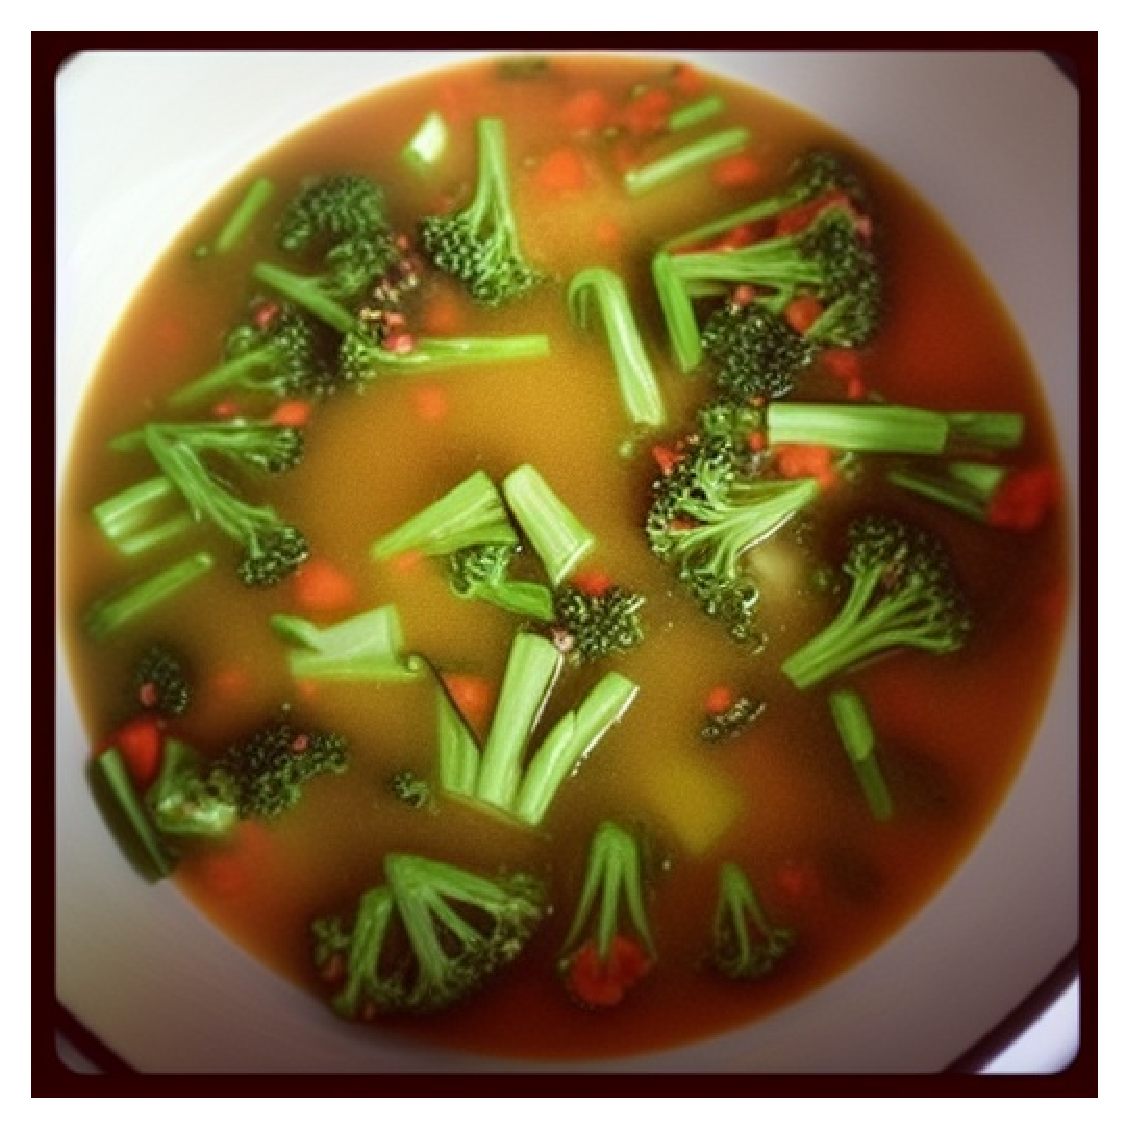
\includegraphics[width=\linewidth]{Ours_compare/58.pdf}
    \end{minipage} &
    \begin{minipage}{\linewidth}
        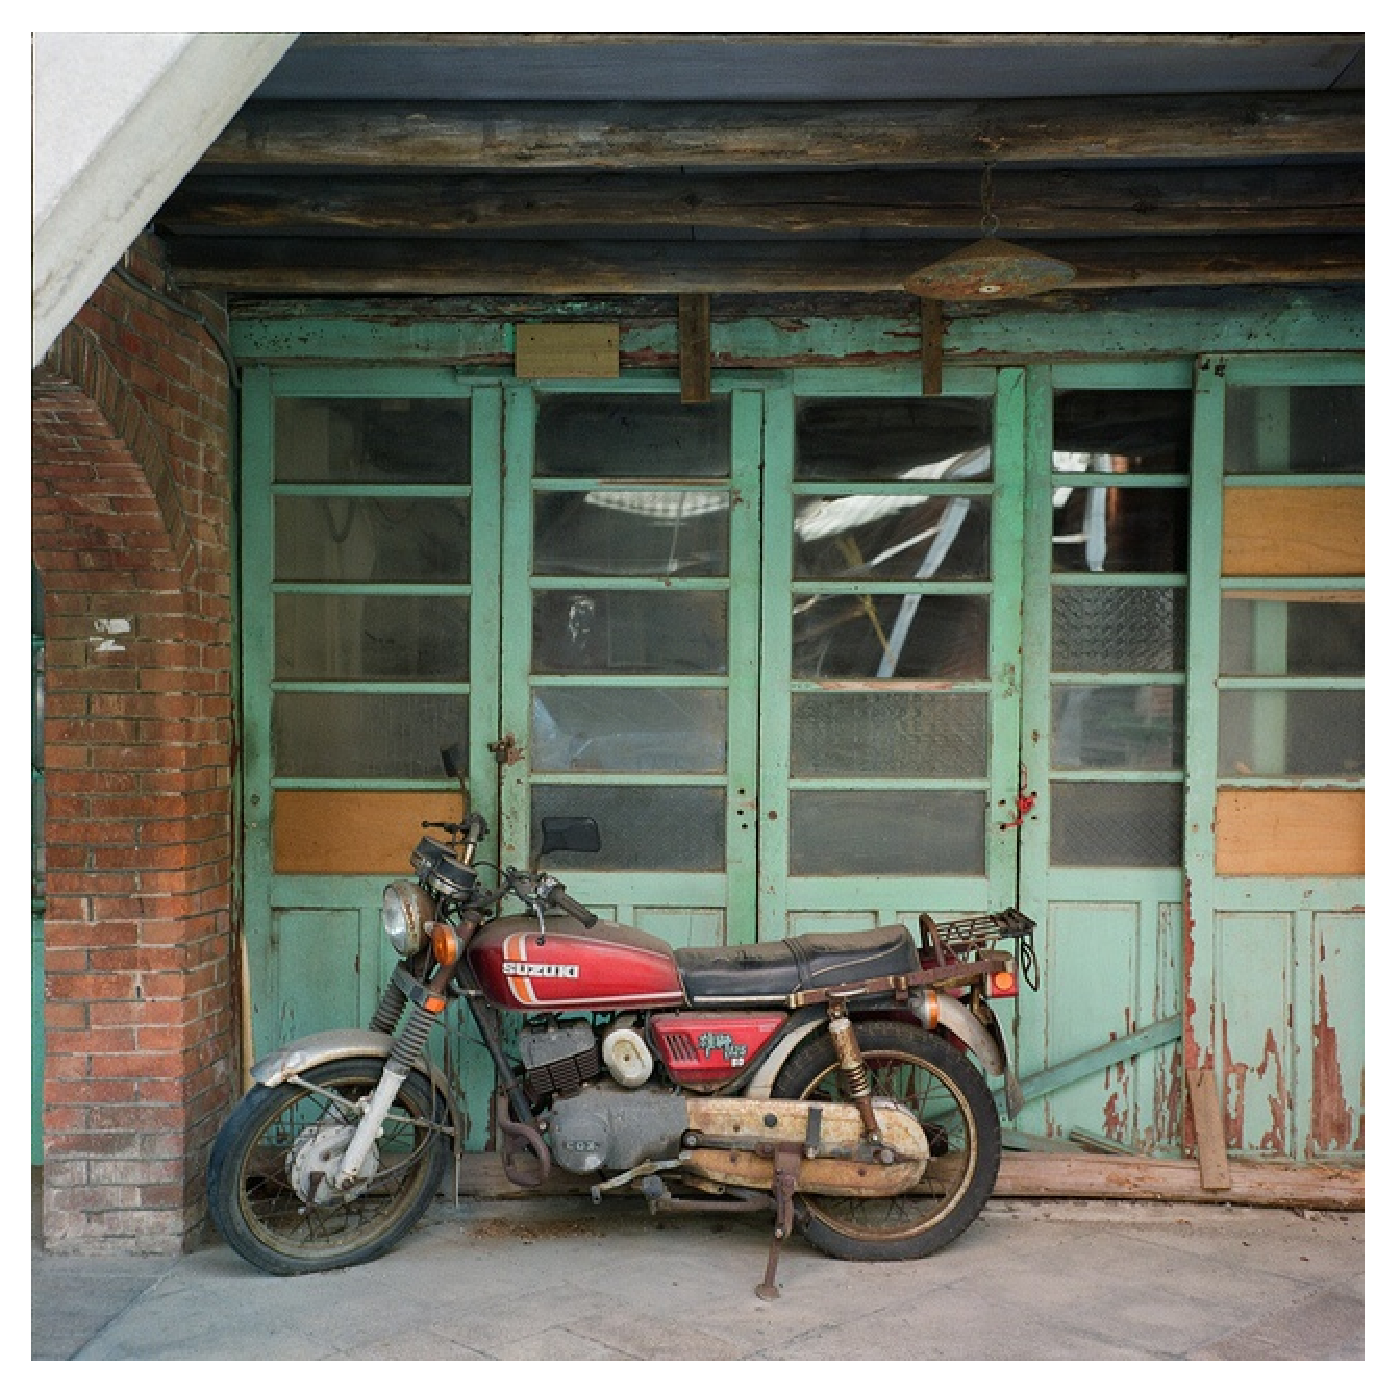
\includegraphics[width=\linewidth]{original_compare/65.pdf}
    \end{minipage} &
    \begin{minipage}{\linewidth}
        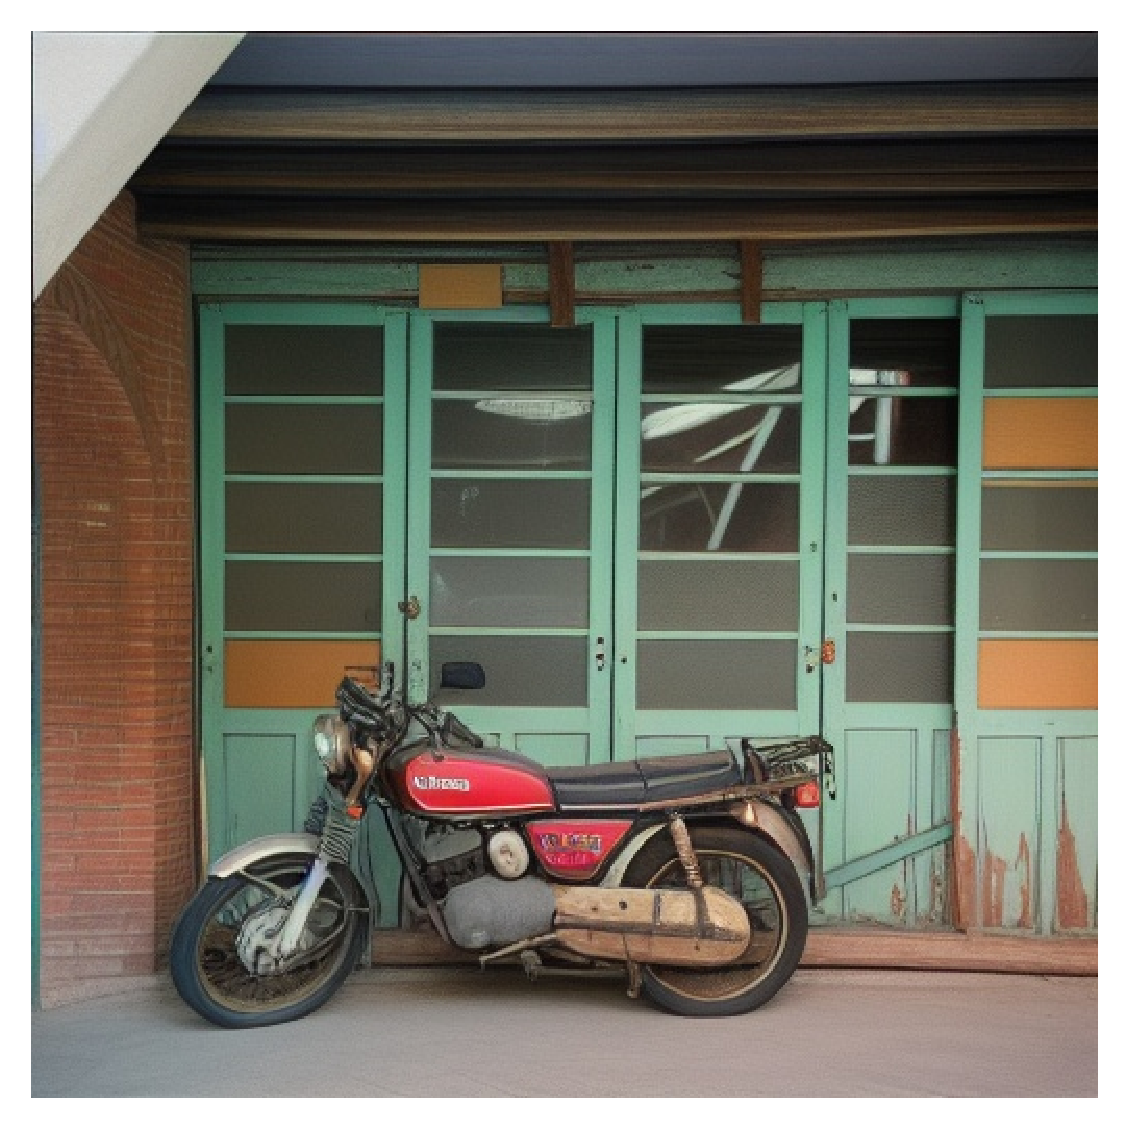
\includegraphics[width=\linewidth]{Ours_compare/65.pdf}
    \end{minipage}
    \\
    \begin{minipage}{\linewidth}
        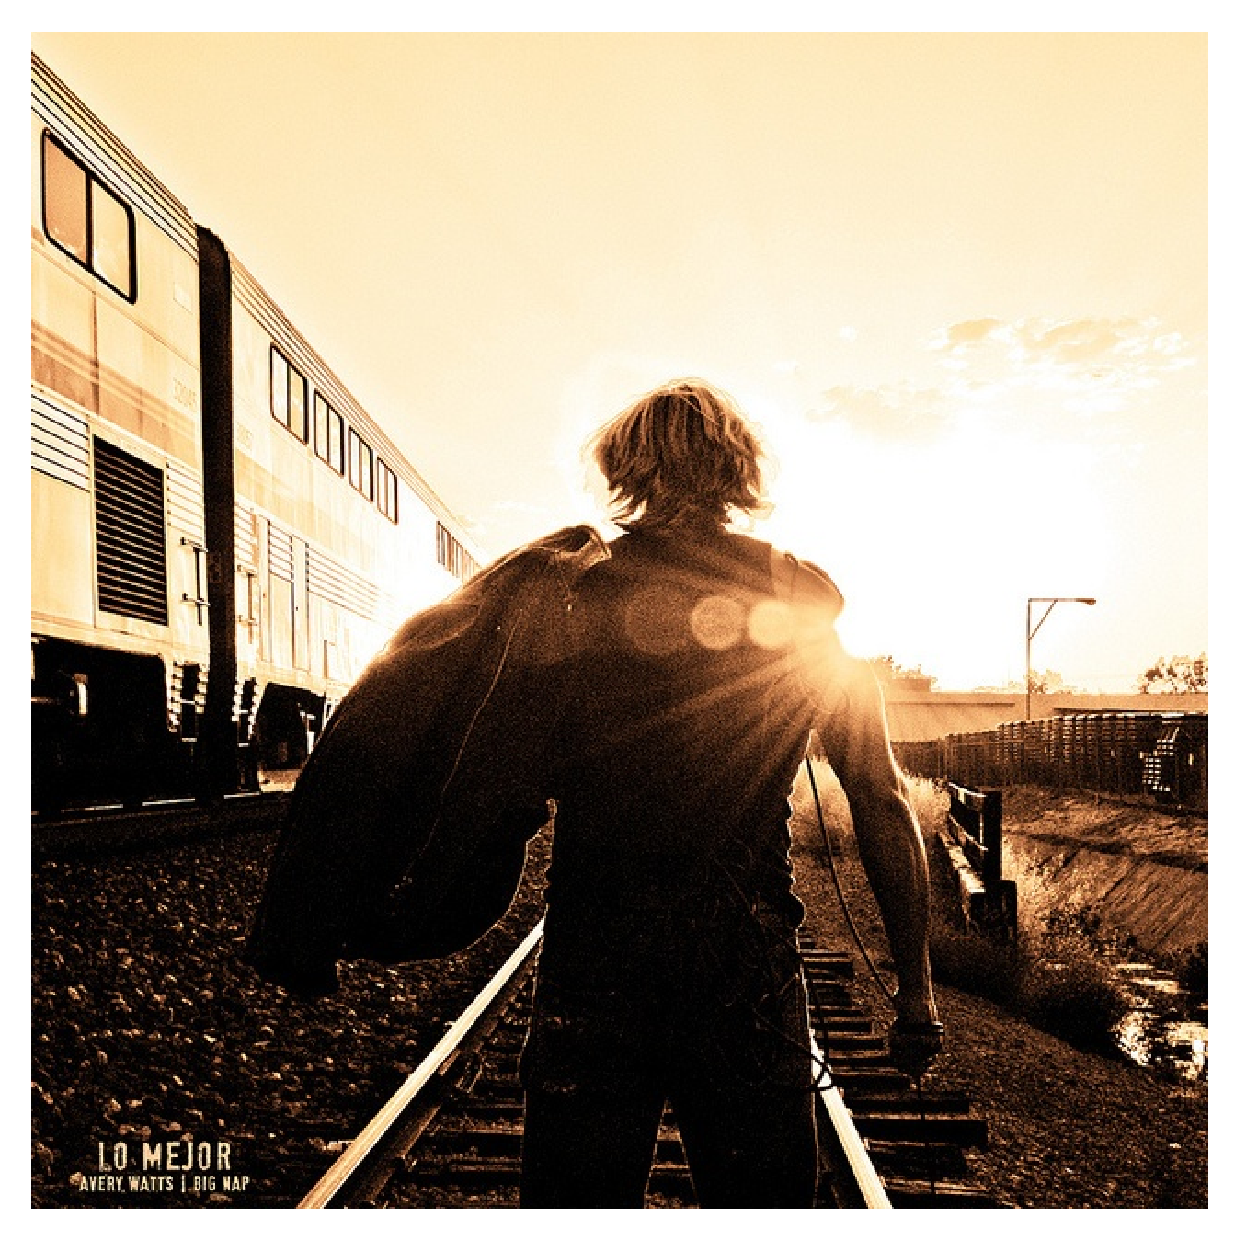
\includegraphics[width=\linewidth]{original_compare/90.pdf}
        \captionof*{figure}{Original image}
    \end{minipage} &
    \begin{minipage}{\linewidth}
        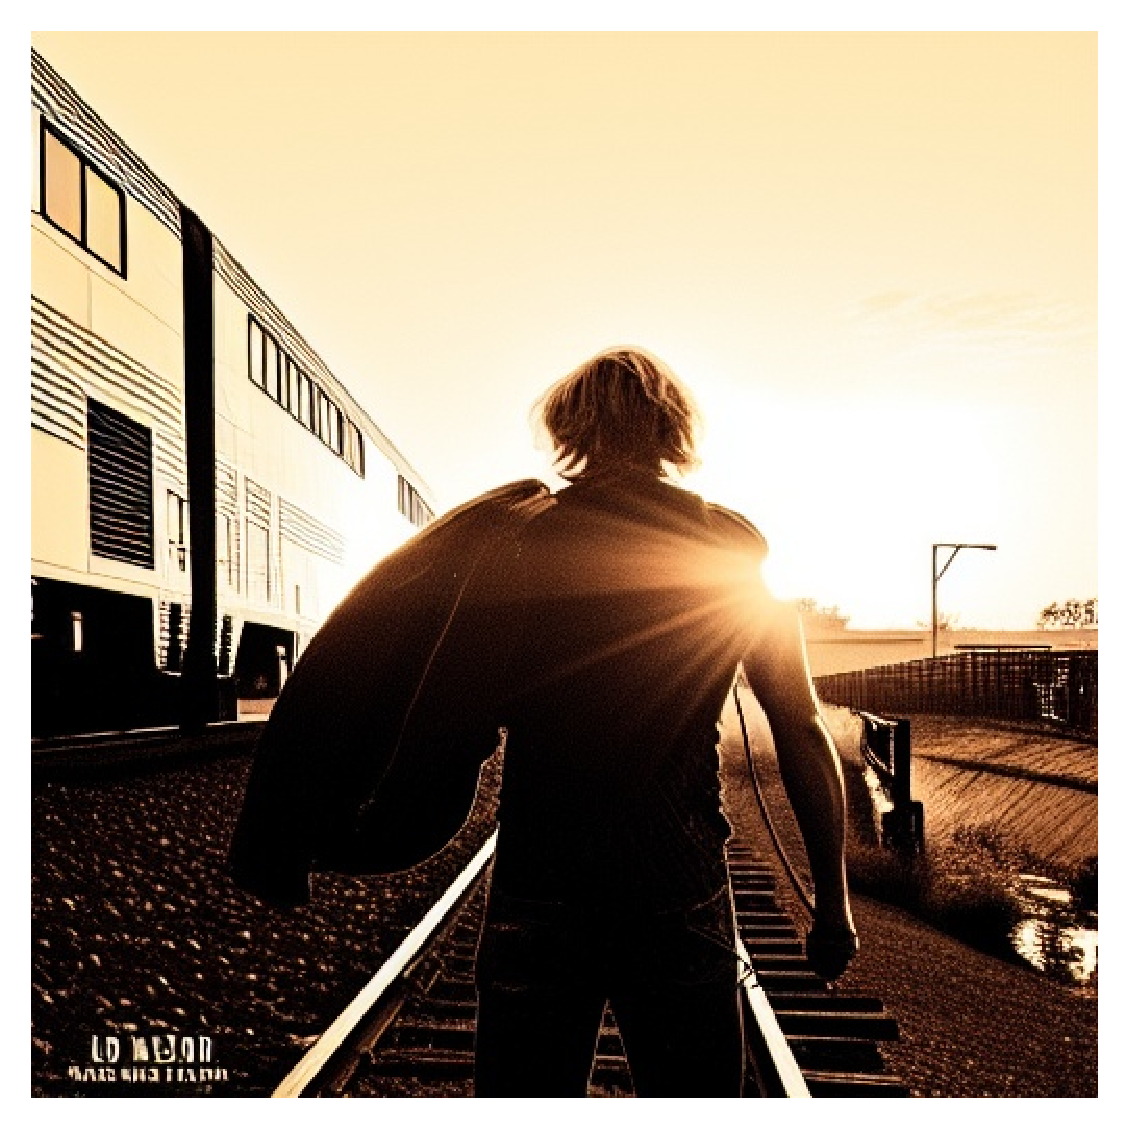
\includegraphics[width=\linewidth]{Ours_compare/90.pdf}
        \captionof*{figure}{EasyInv (Ours)}
    \end{minipage} &
    \begin{minipage}{\linewidth}
        \includegraphics[width=\linewidth]{original_compare/1709.pdf}
        \captionof*{figure}{Original image}
    \end{minipage} &
    \begin{minipage}{\linewidth}
        \includegraphics[width=\linewidth]{Ours_compare/1709.pdf}
        \captionof*{figure}{EasyInv (Ours)}
    \end{minipage}
\end{tabular}
\caption{More visual results of our EasyInv utilizing the SD-V1-4 model.}
\label{fig:compare_more}
\end{figure*}



\subsection{Qualitative Results}
\label{sec:qualitative}
%
We visually evaluate all methods using SD-XL and SD-V1-4. Figure\,\ref{SDXL_compare} presents a comparison of several examples across all methods utilizing SD-XL. ReNoise struggles with images containing significant white areas, resulting in black images. The other two methods also perform poorly, especially evident in the clock example.
%
Figure\,\ref{SDV1-4_compare} displays the results obtained from the SD-V1-4 using images sourced from the internet. These images also feature large areas of white color. ReNoise consistently produces black images with these inputs, indicating an issue inherent to the method rather than the model. Fixed-Point Iteration and DDIM Inversion also fail to generate satisfactory results in such cases, suggesting these images pose challenges for inversion methods. Our method, shown in the figure, effectively addresses these challenges, demonstrating robustness and enhancing performance in handling special scenarios.
%
These findings underscore the efficacy of our approach, particularly in addressing challenging cases that are less common in the COCO dataset. 




Figure~\ref{fig:compare_more} presents more visual results of our method, with original images exclusively obtained from the COCO dataset~\cite{COCO}. The results are unequivocal: our approach consistently generates images that closely resemble their originals post-inversion and reconstruction. The variety of categories represented in these images underscores the broad applicability and consistent performance of our method. In aggregate, these findings affirm that our technique is not merely efficient but also remarkably robust, adeptly reconstructing images with a high level of precision and clarity.


\begin{figure}[!t]
    \centering
    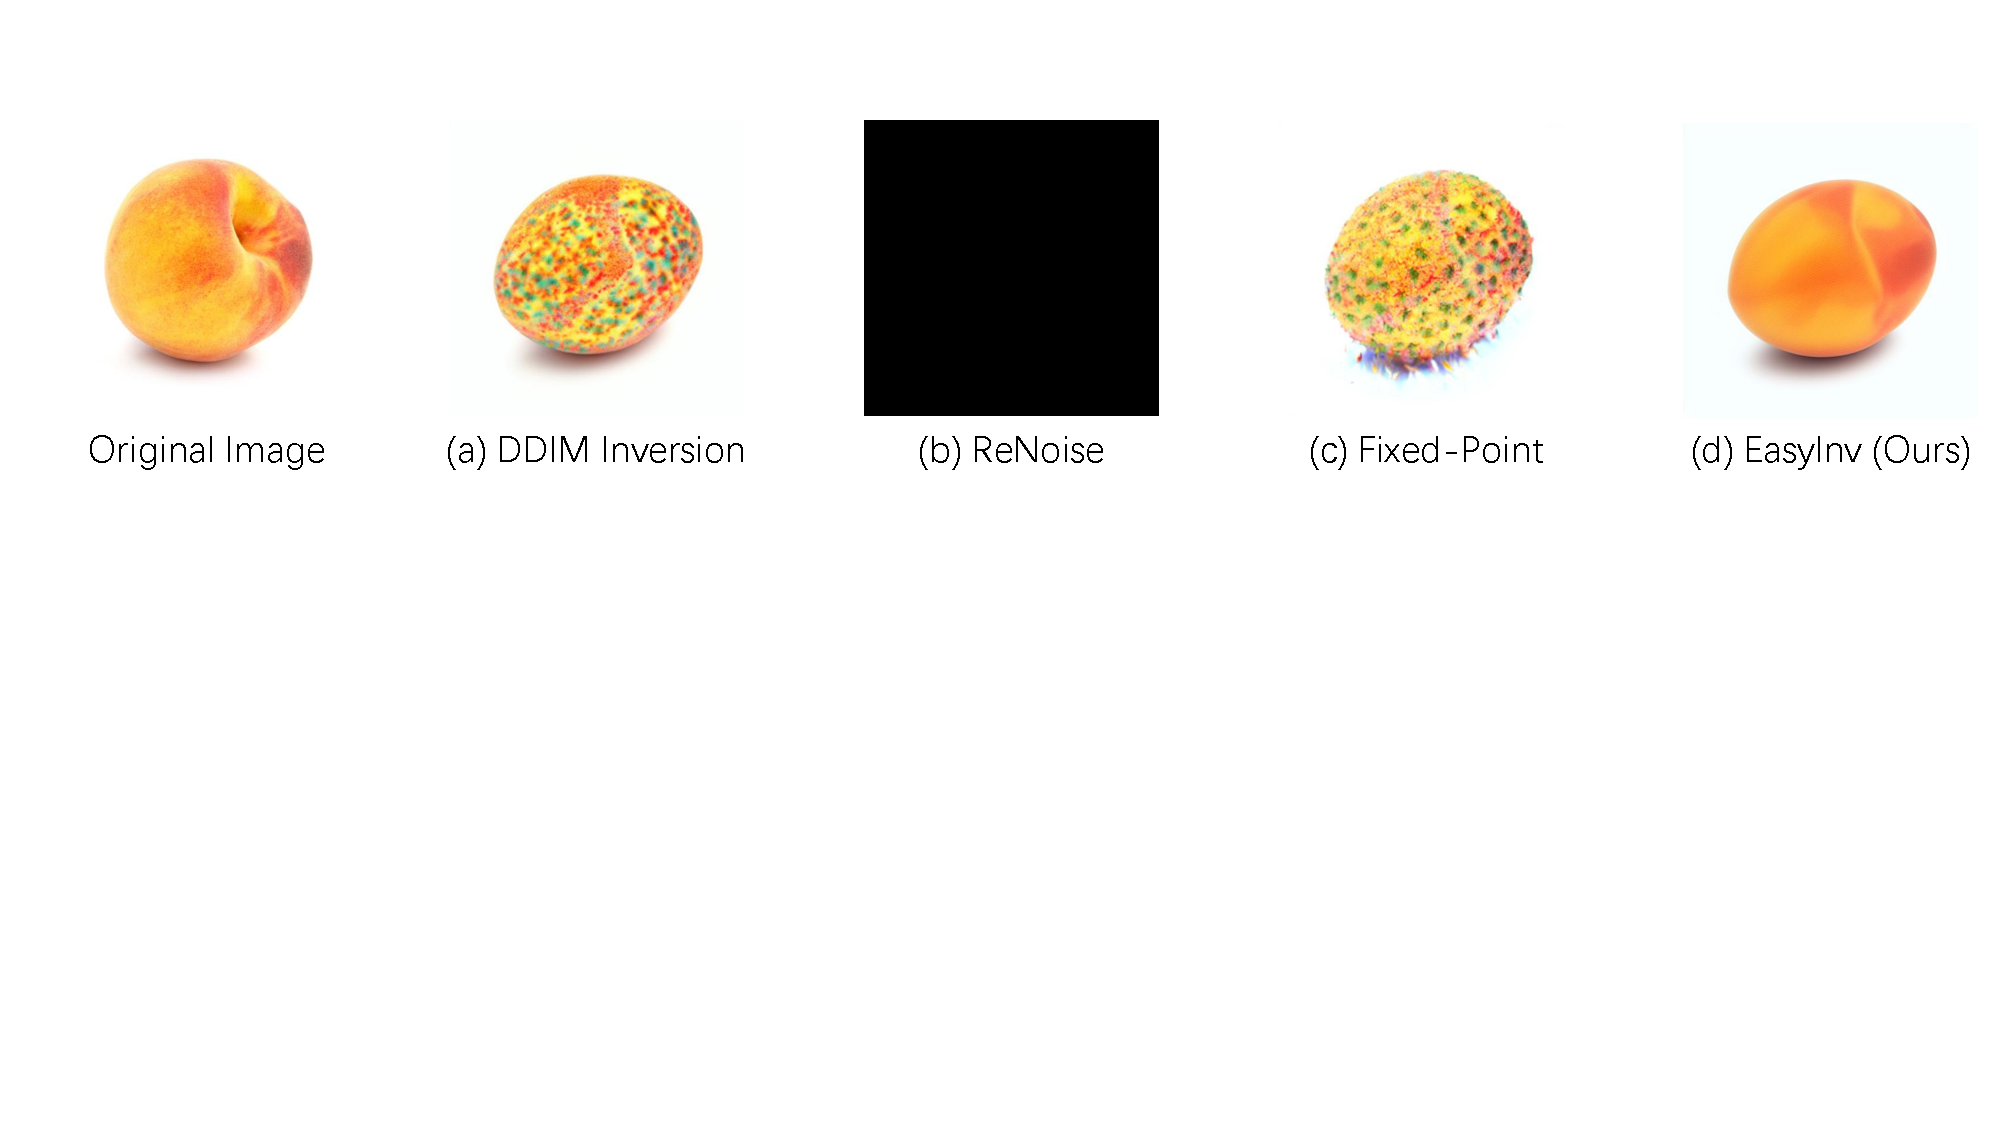
\includegraphics[width=0.98\linewidth]{visual_masa_cut.pdf}
    \caption{Results of MasaCtrl~\cite{cao_2023_masactrl} with prompt ``A football'', using inverted latent generated by different methods as input.}
    \label{masa_compare}
\end{figure}



\subsection{Downstream Image Editing}
%
To showcase the practical utility of our EasyInv, we have employed various inversion techniques within the realm of consistent image synthesis and editing. We have seamlessly integrated these inversion methods into MasaCtrl~\cite{cao_2023_masactrl}, a widely-adopted image editing approach that extracts correlated local content and textures from source images to ensure consistency. For demonstrative purposes, we present an image of a ``peach'' alongside the prompt ``A football.'' The impact of inversion quality is depicted in Figure \ref{masa_compare}. In these instances, we utilize the inverted latents of the ``peach'' image, as shown in Figure \ref{SDV1-4_compare}, as the input for MasaCtrl~\cite{cao_2023_masactrl}. Our ultimate goal is to generate an image of a football that retains the distinctive features of the ``peach'' image. As evident from Figure \ref{masa_compare}, our EasyInv achieves superior texture quality and a shape most closely resembling that of a football. From our perspective, images with extensive white areas constitute a significant category in actual image editing, given that they are a prevalent characteristic in conventional photography. However, such features often prove detrimental to the ReNoise method. Thus, for authentic image editing scenarios, our approach stands out as a preferable alternative, not to mention its commendable efficiency.




\subsection{Limitations}
\label{sec:weakness}

One potential risk associated with our approach is the phenomenon known as ``over-denoising,'' which occurs when there is a disproportionate focus on achieving a pristine final-step latent state. This can occasionally result in overly smooth image outputs, as exemplified by the ``peach'' figure in Figure\,\ref{SDV1-4_compare}.
%
In the context of most real-world image editing tasks, this is not typically an issue, as these tasks often involve style migration, which inherently alters the details of the original image. However, in specific applications, such as using diffusion models for creating advertisements, this could pose a challenge.
%
Nonetheless, our experimental results highlight that the method's two key benefits significantly outweigh this minor shortcoming. Firstly, it is capable of delivering satisfactory outcomes even with models that may under-perform relative to other methods, as shown in the above experiments. Secondly, it enhances inversion efficiency by reverting to the original DDIM Inversion baseline~\cite{couairon2023diffedit}, thereby eliminating the necessity for iterative optimizations. This strategy not only simplifies the process but also ensures the maintenance of high-quality outputs, marking it as a noteworthy advancement over current methodologies. 


In conclusion, our research has made significant strides with the introduction of EasyInv. As we look ahead, our commitment to advancing this technology remains unwavering. Our future research agenda will be focused on the persistent enhancement and optimization of the techniques in this paper. This will be done with the ultimate goal of ensuring that our methodology is not only robust and efficient but also highly adaptable to the diverse and ever-evolving needs of industrial applications.

\section{Conclusion}
Our EasyInv presents a significant advancement in the field of DDIM Inversion by addressing the inefficiencies and performance limitations in traditional iterative optimization methods. By emphasizing the importance of the initial latent state and introducing a refined strategy for approximating inversion noise, EasyInv enhances both the accuracy efficiency of the inversion process. Our method strategically reinforces the initial latent state's influence, mitigating the impact of noise and ensuring a closer reconstruction to the original image. This approach not only matches but often surpasses the performance of existing DDIM Inversion methods, especially in scenarios with limited model precision or computational resources. EasyInv also demonstrates a remarkable improvement in inference efficiency, achieving approximately three times faster processing than standard iterative techniques. Through extensive evaluations, we have shown that EasyInv consistently delivers high-quality results, making it a robust and efficient solution for image inversion tasks. The simplicity and effectiveness of EasyInv underscore its potential for broader applications, promoting greater accessibility and advancement in the field of diffusion models.



































\bibliography{aaai25}

\end{document}
